\chapter{Results}\label{section:star_results}
In the following section, the  final-state charged particle distributions are compared with various  SD MC predictions, i.e. 
\begin{itemize}
	\item PYTHIA 8 4C (SaS),
	\item PYTHIA 8 A2 (MBR),
	\item PYTHIA 8 A2 (MBR-tuned),
	\item HERWIG 7,
	\item EPOS LHC with combined two classes of processes: diffractive (EPOS SD) and non-diffractive (EPOS SD$^\prime$),
	\item EPOS LHC SD$^\prime$.
\end{itemize}

\begin{figure}[b!]
	\centering
	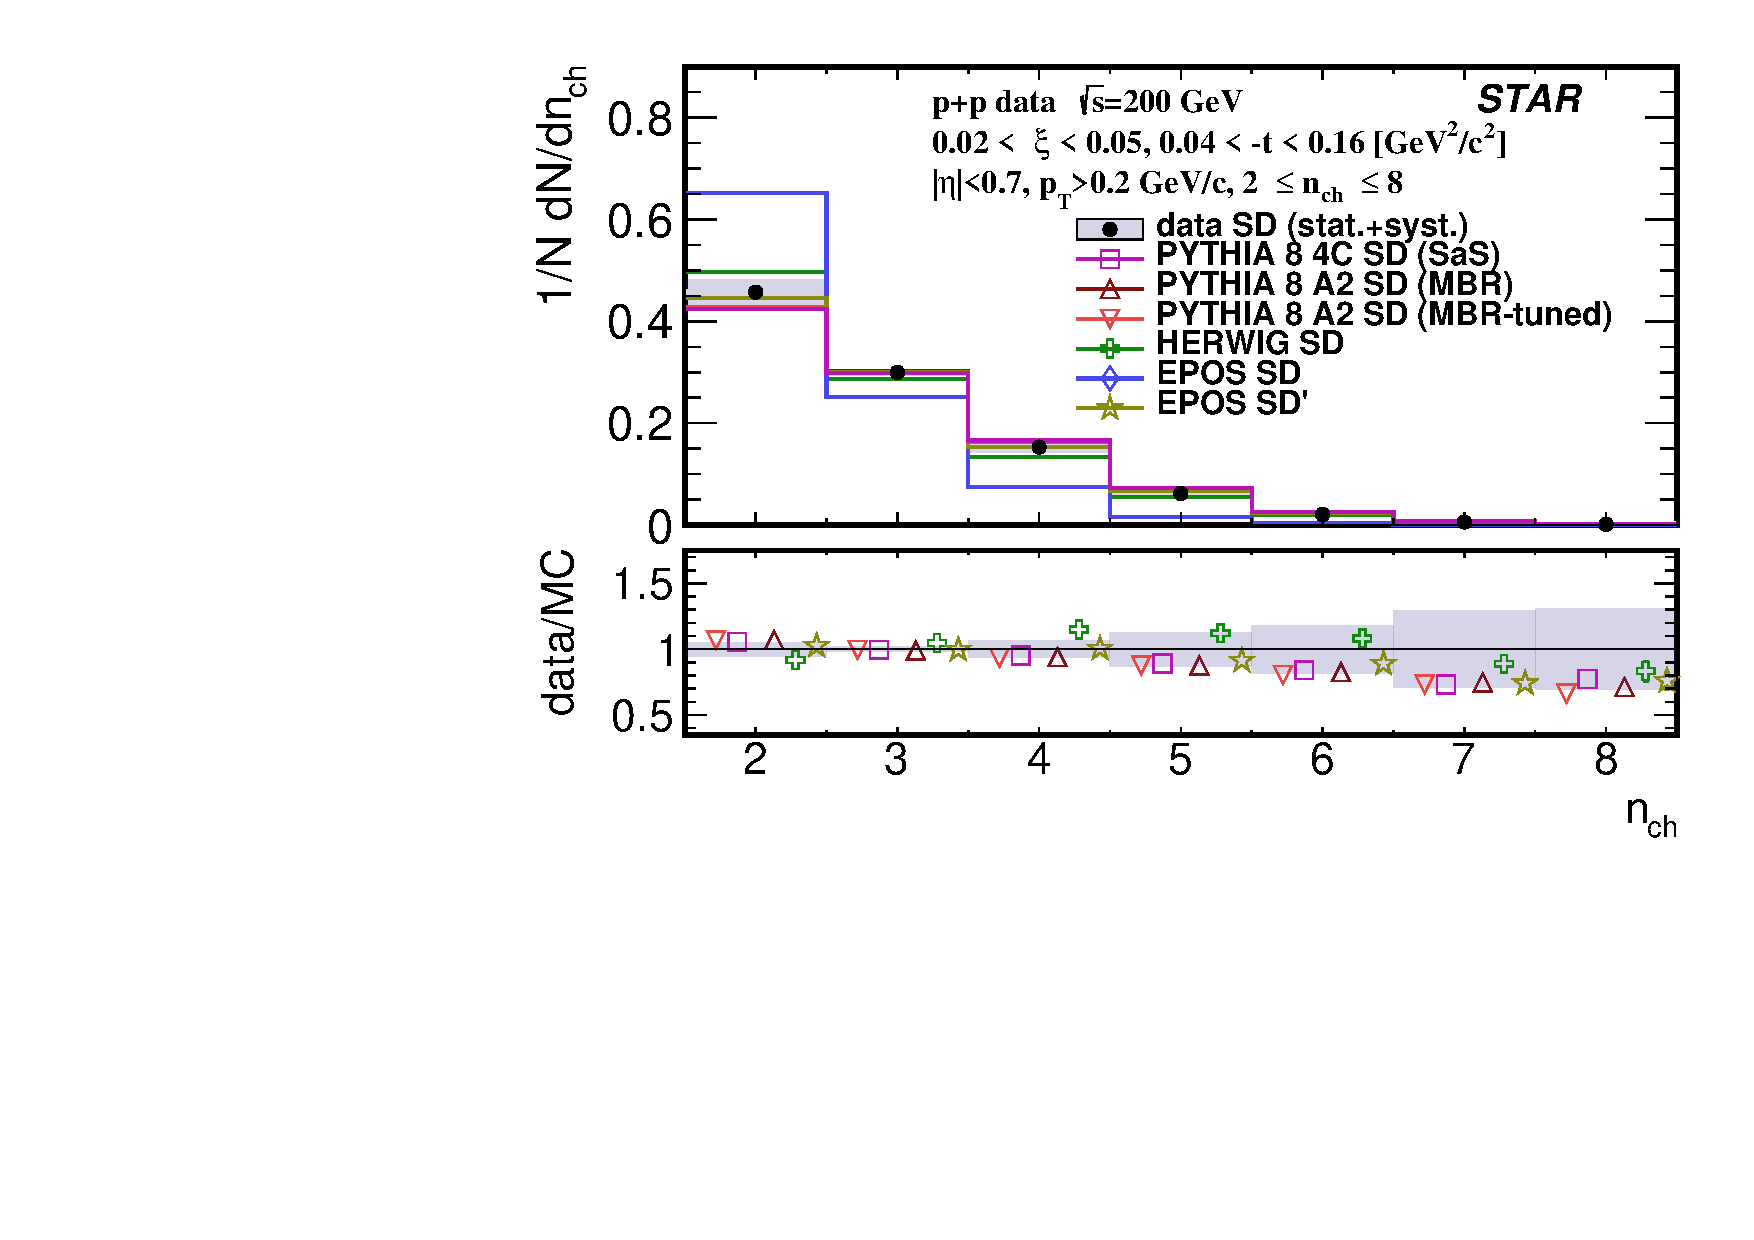
\includegraphics[width=.49\textwidth,page=1]{chapters/chrgSTAR/img/results/nch_ksi_0.pdf}
	\hfill
	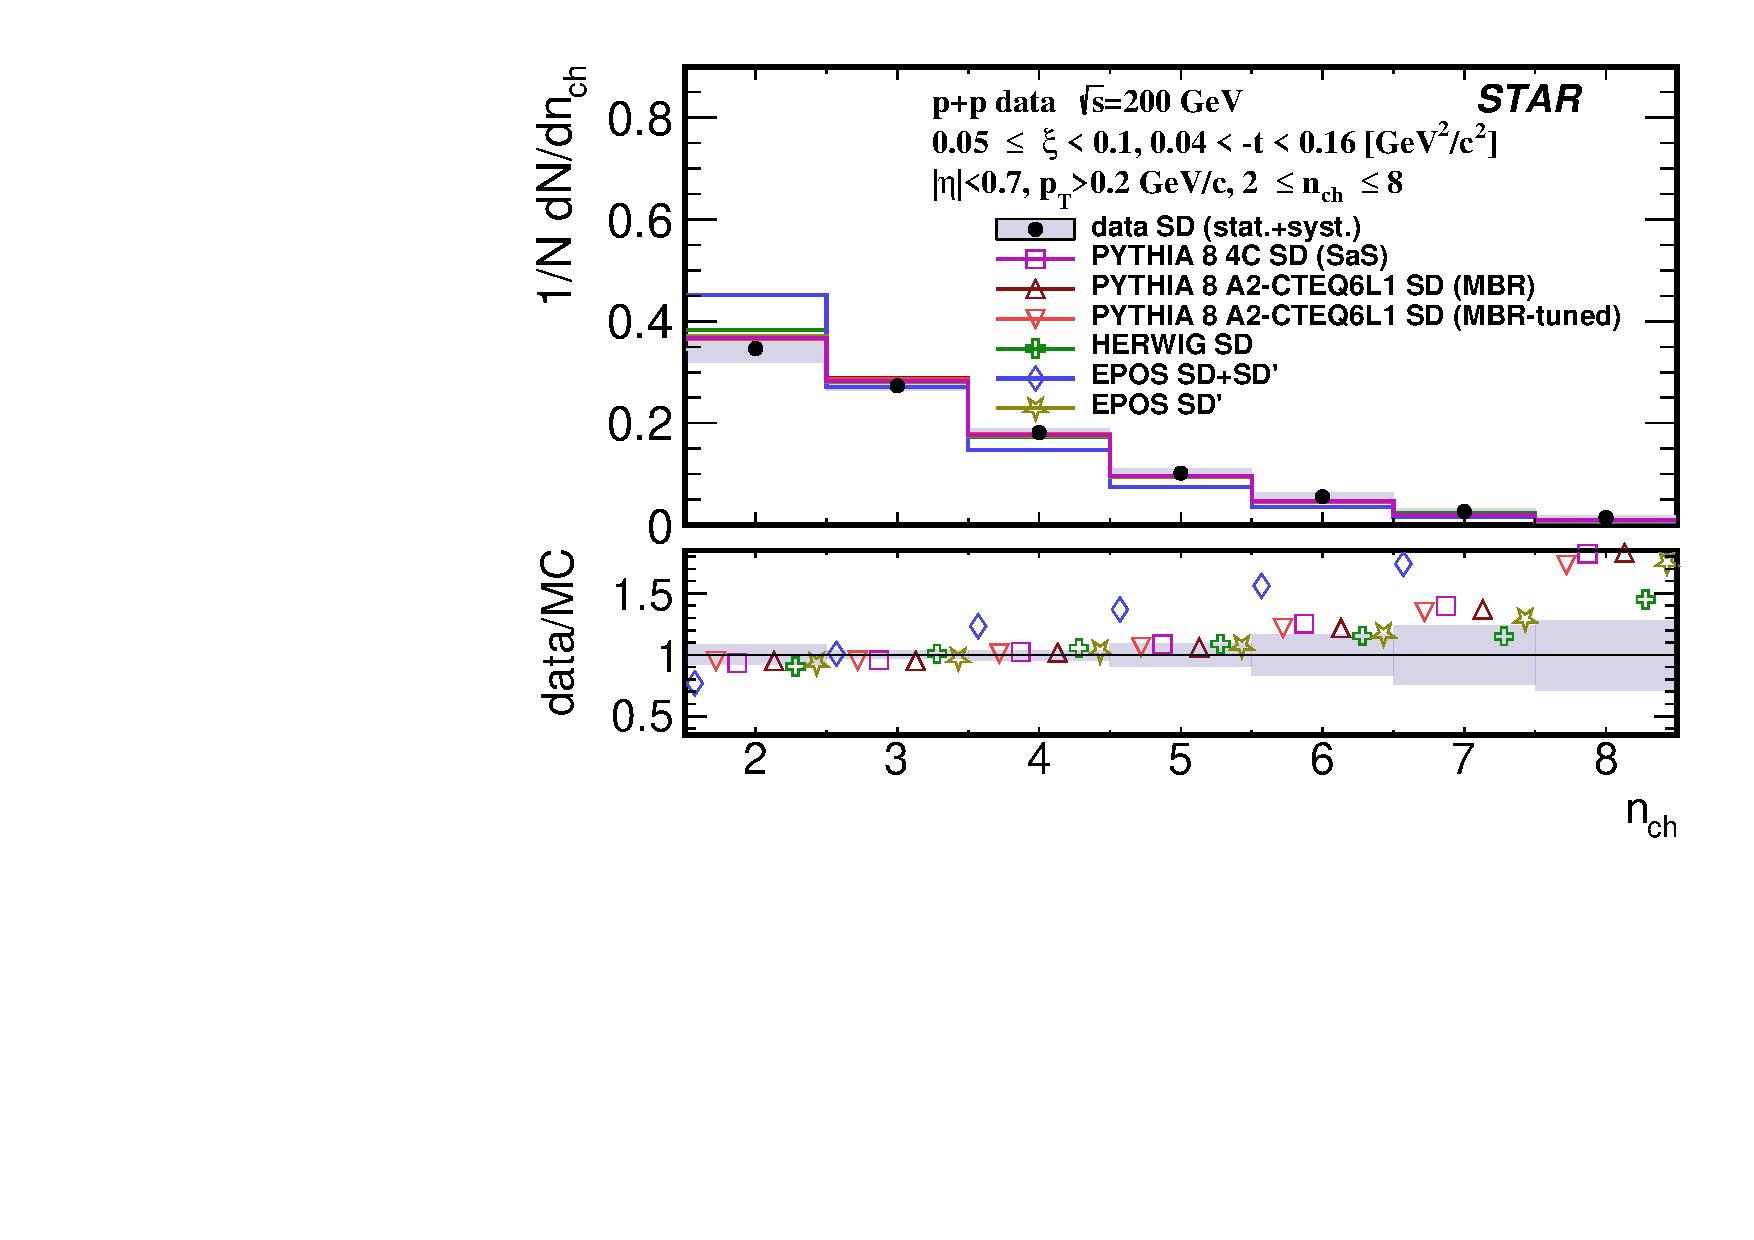
\includegraphics[width=.49\textwidth,page=1]{chapters/chrgSTAR/img/results/nch_ksi_1.pdf}
	\newline
	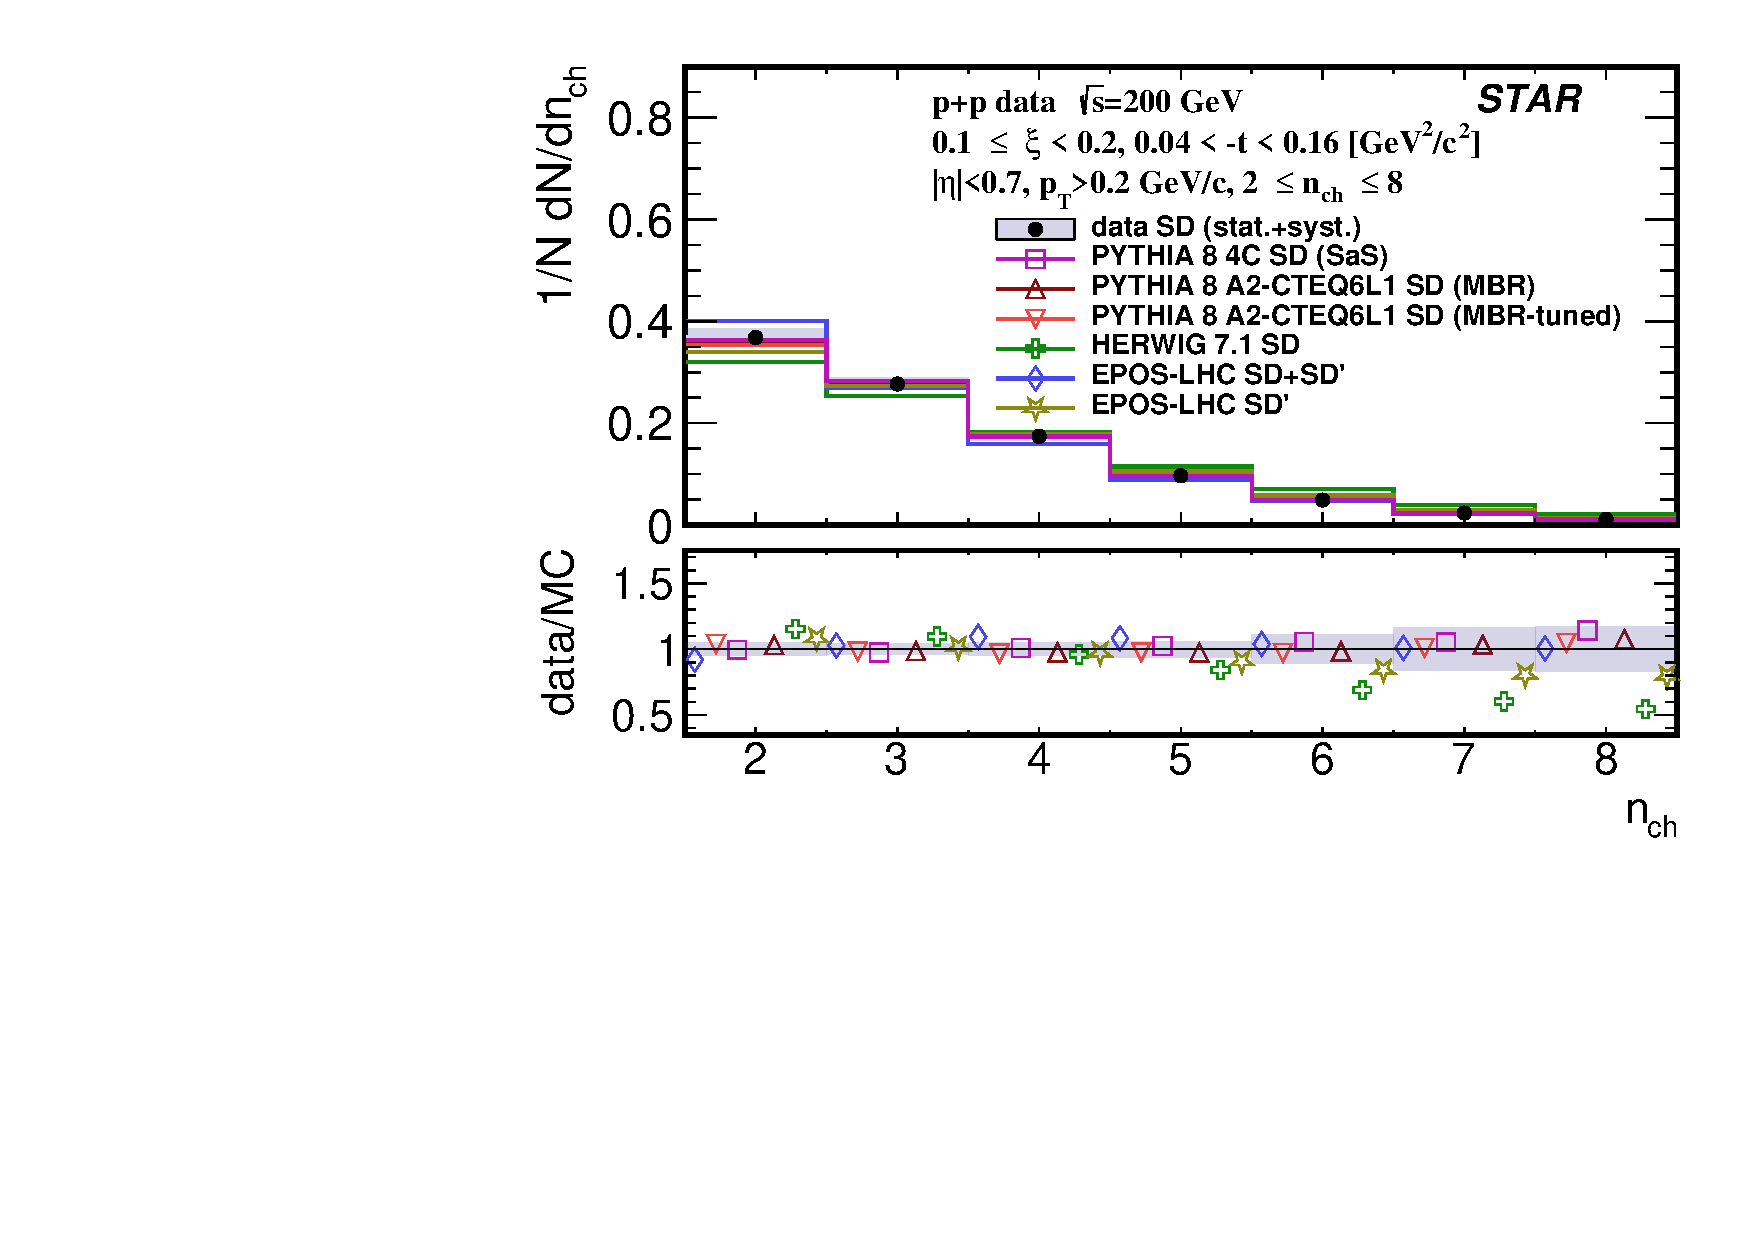
\includegraphics[width=.49\textwidth,page=1]{chapters/chrgSTAR/img/results/nch_ksi_2.pdf}
	\hfill
	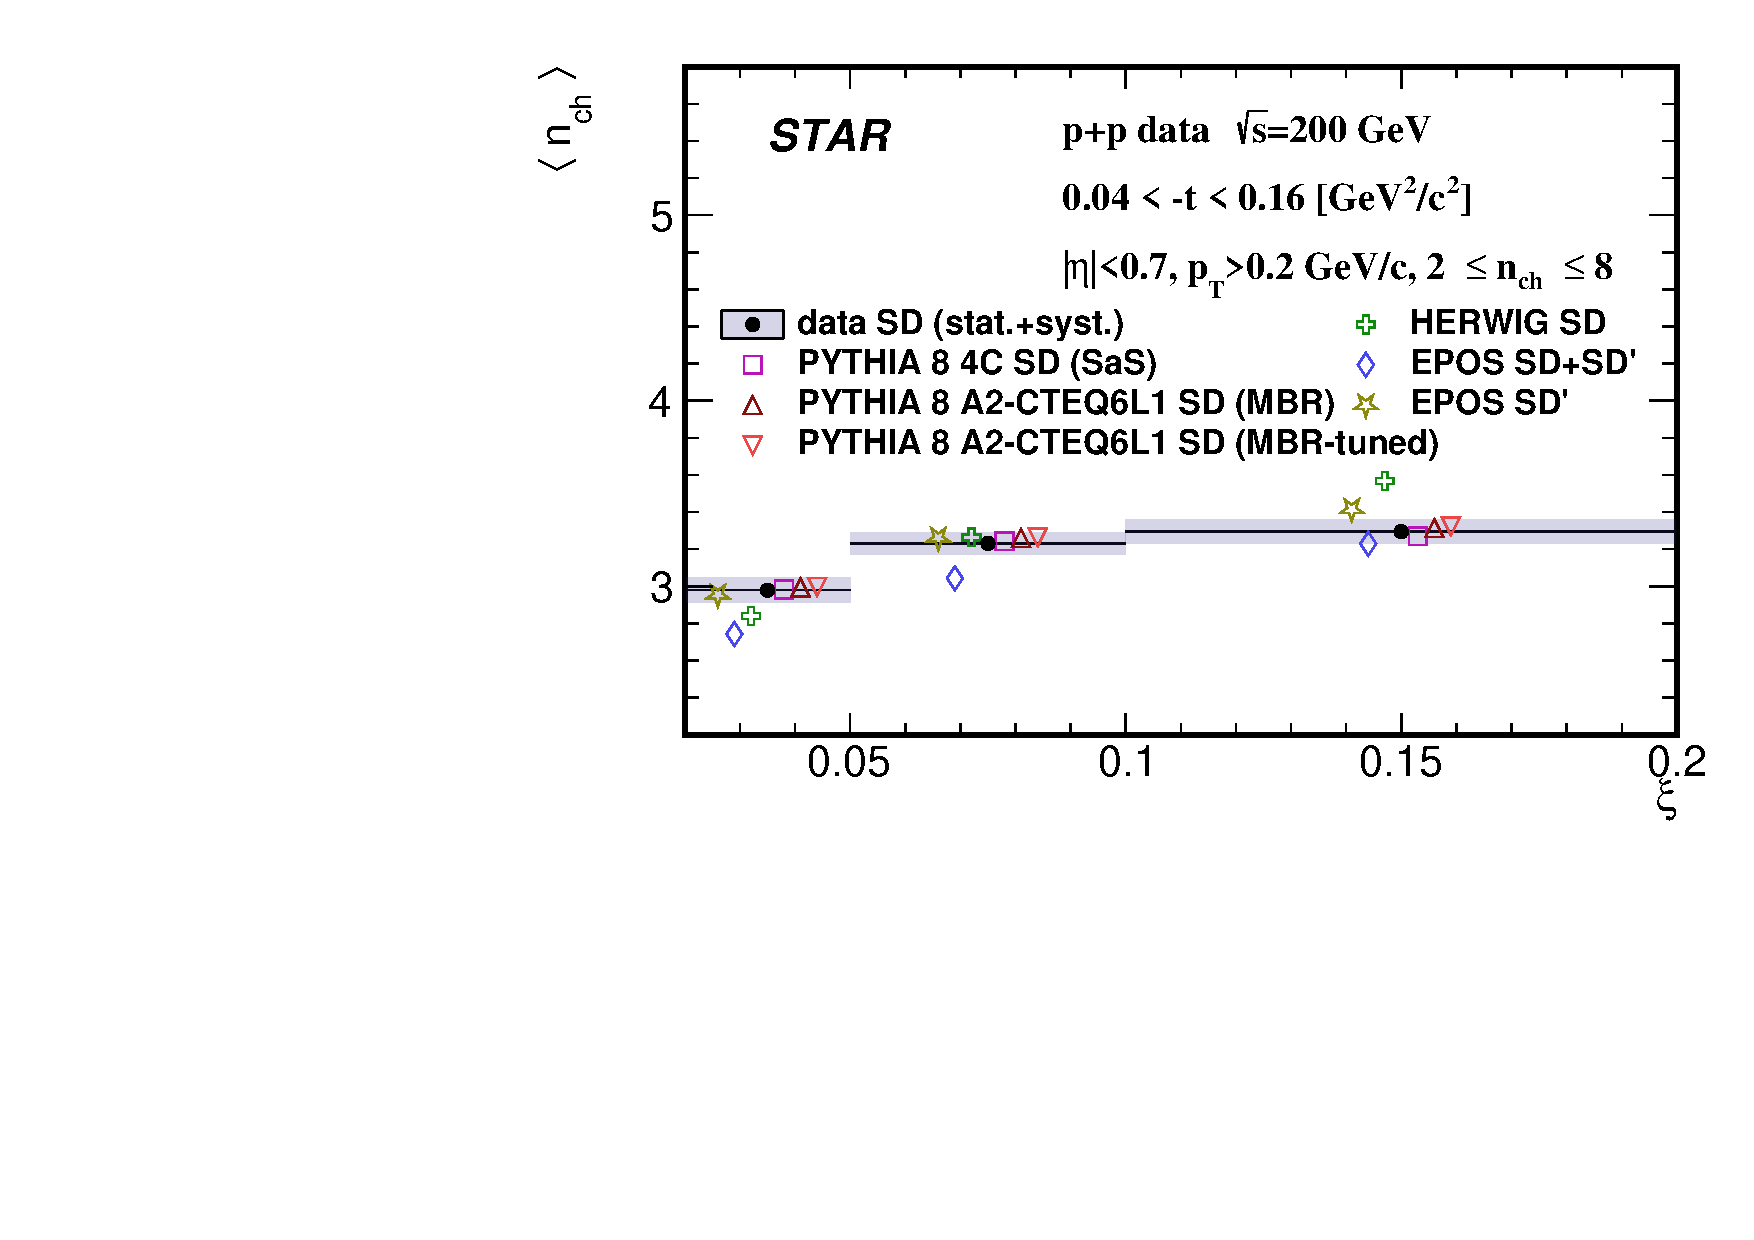
\includegraphics[width=.49\textwidth,page=1]{chapters/chrgSTAR/img/results/mean_nch_xi.pdf}
	%
	\caption{Primary charged-particle multiplicity shown separately for the~three ranges of  $\xi$: (top left) $0.02<\xi<0.05$, (top right) $0.05<\xi<0.1$, (bottom left) $0.1<\xi<0.2$ and (bottom right) the mean multiplicity $\langle n_\textrm{ch}\rangle$ as a function of $\xi$.}
	\label{fig:results_star_nch}
\end{figure}
In all figures, data are shown as solid points with error bars representing the statistical uncertainties. Gray boxes represent statistical and systematic uncertainties added in quadrature. Predictions from MC models are shown as colour histograms and markers. The~lower panel in each figure shows the ratio of data to the models' predictions. All results are presented separately for three ranges of $\xi$: $0.02 < \xi<0.05$, $0.05<\xi<0.1$, $0.1<\xi<0.2$.

In Fig.~\ref{fig:results_star_nch} we show multiplicity distributions of charged particles in different intervals of $\xi$ as well as the average values of $_\textrm{ch}$ in those $\xi$ ranges. 
Data exhibit an expected increase of the $\langle n_\textrm{ch}\rangle$ with $\xi$ due to the larger diffractive masses probed at increasing $\xi$ in SD process. The shapes of the measured distributions are reproduced reasonably well by all models except the EPOS SD+SD$^\prime$, which predicts much smaller $\langle n_\textrm{ch}\rangle$ at $\xi<0.1$ and the HERWIG SD, which for $0.1<\xi<0.2$ predicts too large $\langle n_\textrm{ch}\rangle$.
It should be noted, that EPOS SD$^\prime$ describes data much better compared to EPOS SD+SD$^\prime$.

%HERWIG-SD which for $0.1<\xi<0.2$ predicts too large $\langle n_\textrm{ch}\rangle$.
\begin{figure}[b!]
	\centering
	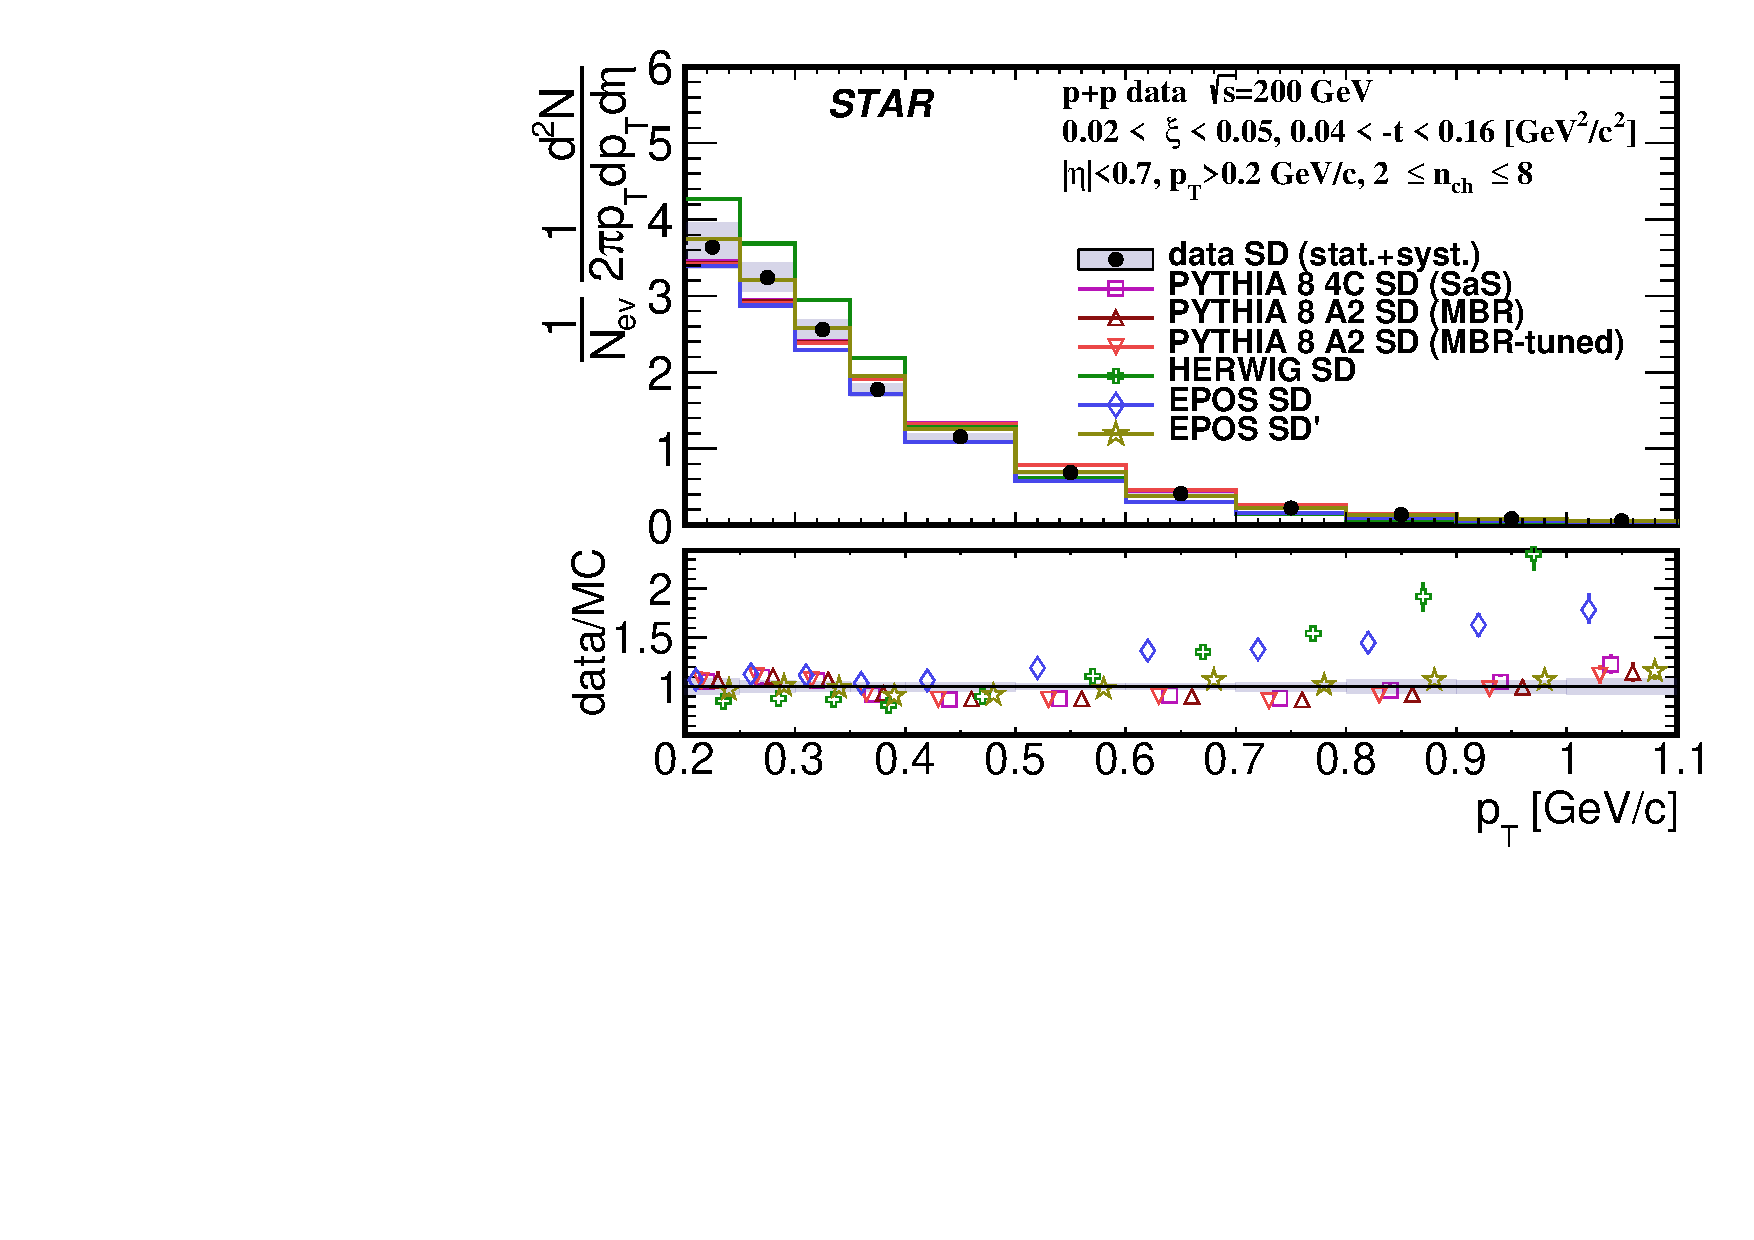
\includegraphics[width=.49\textwidth,page=1]{chapters/chrgSTAR/img/results/out_pt_ksi_0.pdf}
	\hfill
	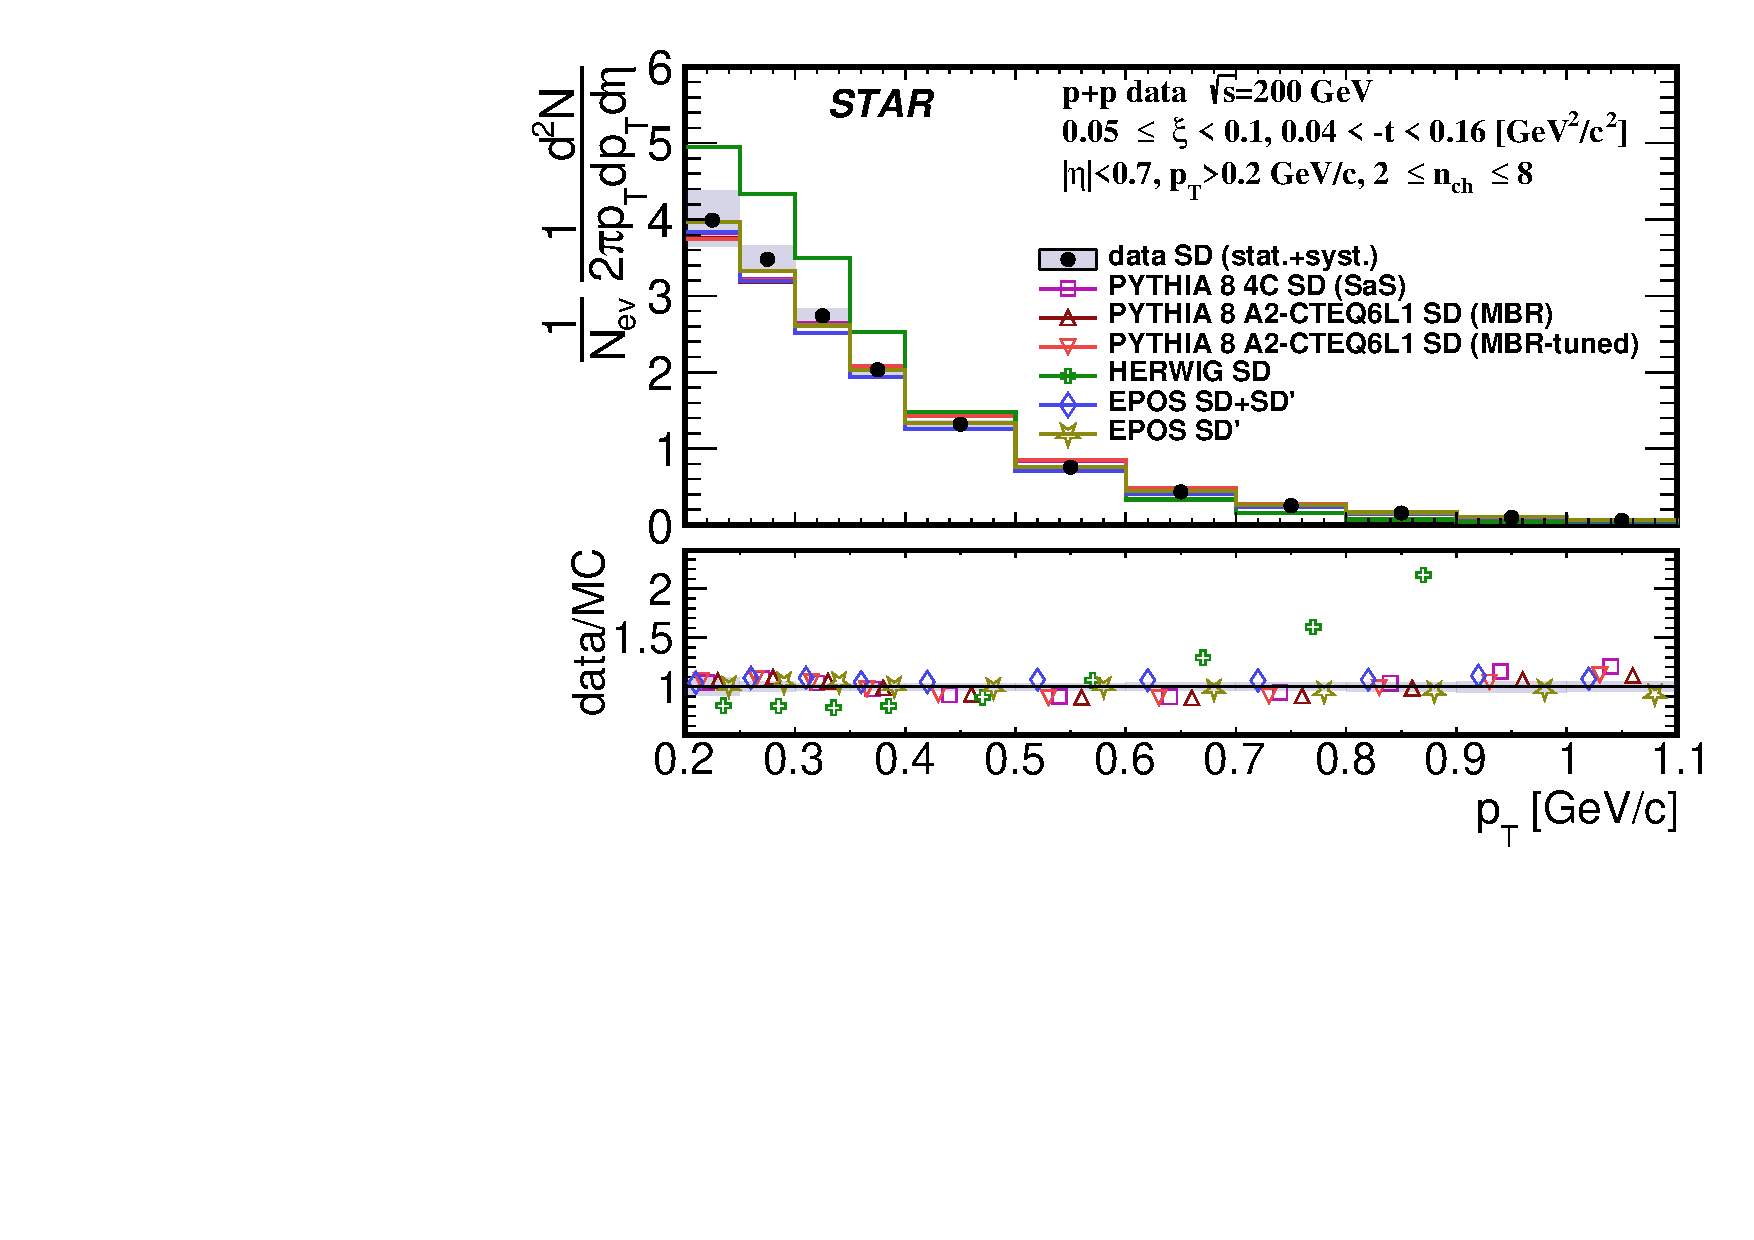
\includegraphics[width=.49\textwidth,page=1]{chapters/chrgSTAR/img/results/out_pt_ksi_1.pdf}
	\newline
	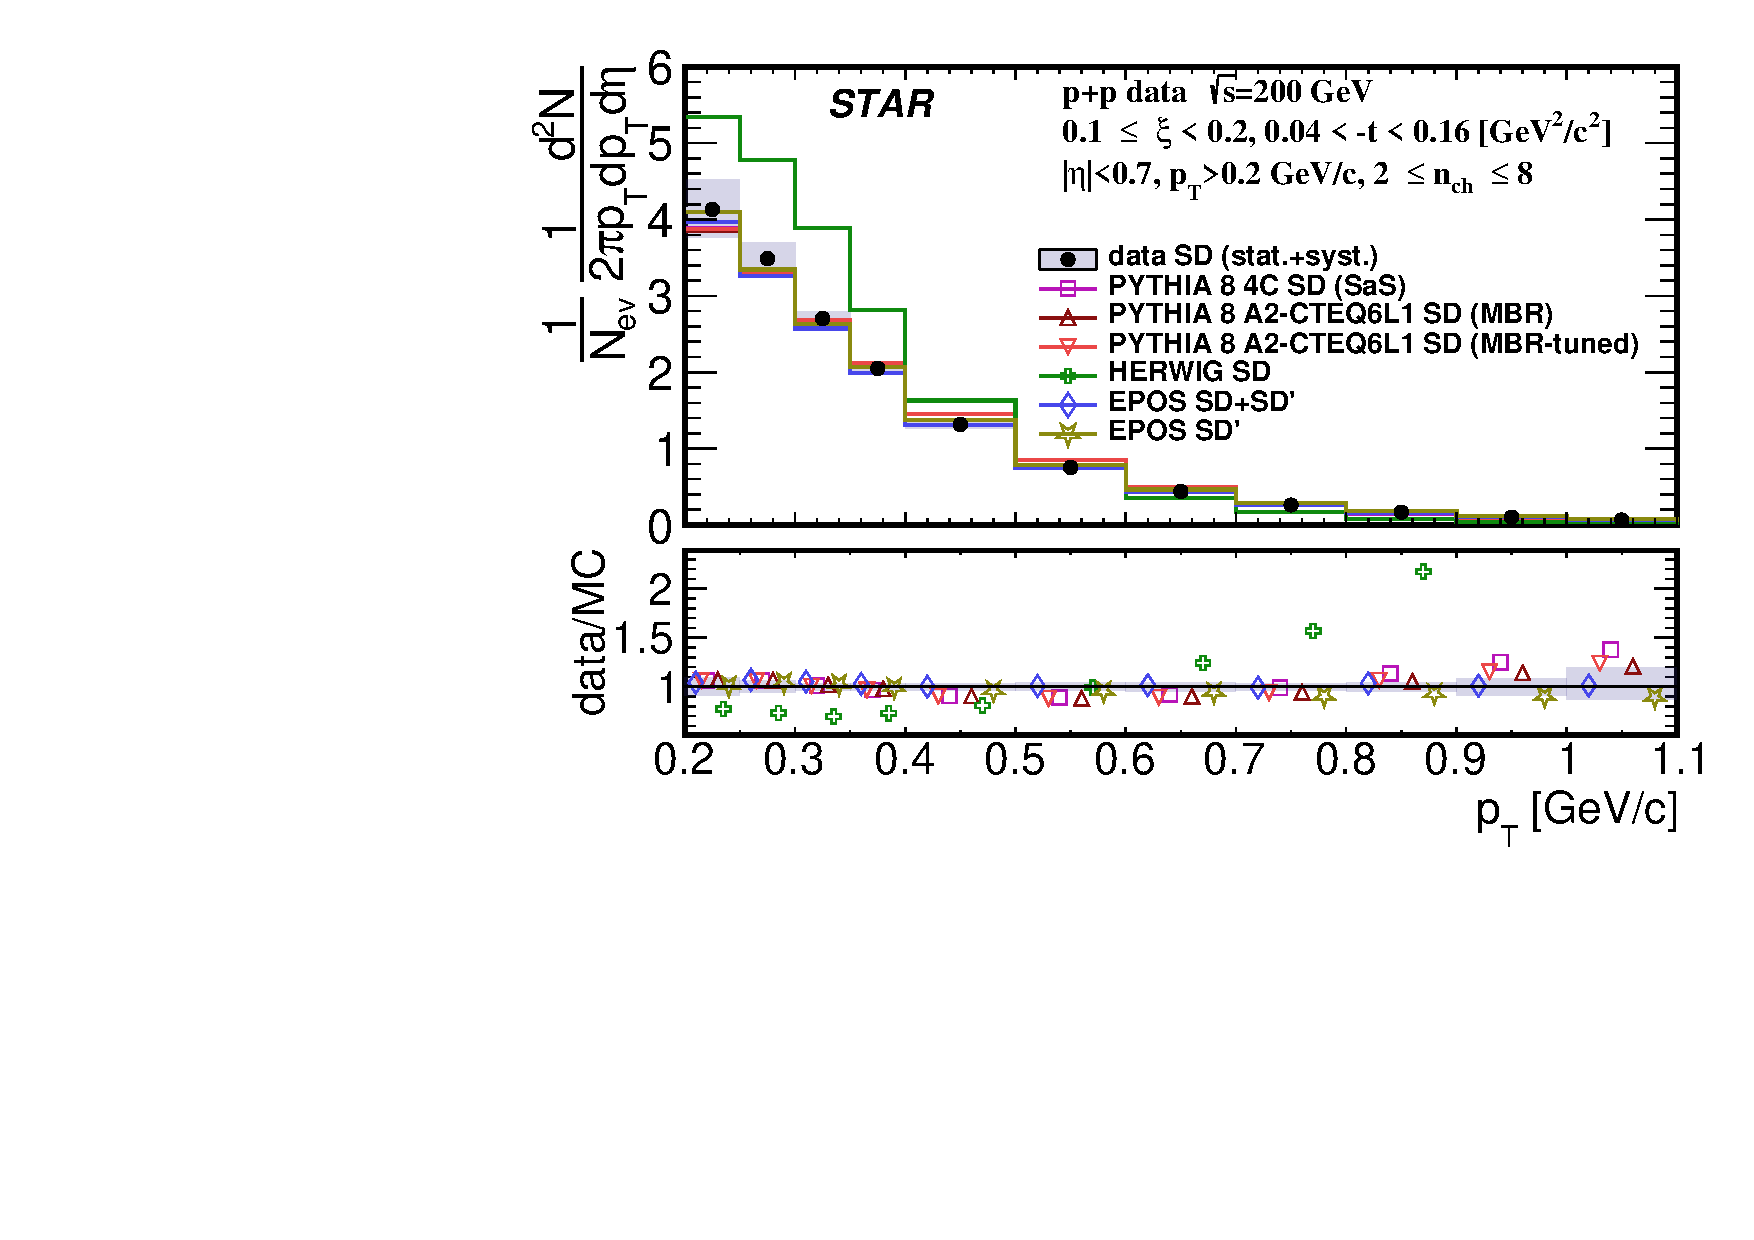
\includegraphics[width=.49\textwidth,page=1]{chapters/chrgSTAR/img/results/out_pt_ksi_2.pdf}
	\hfill
	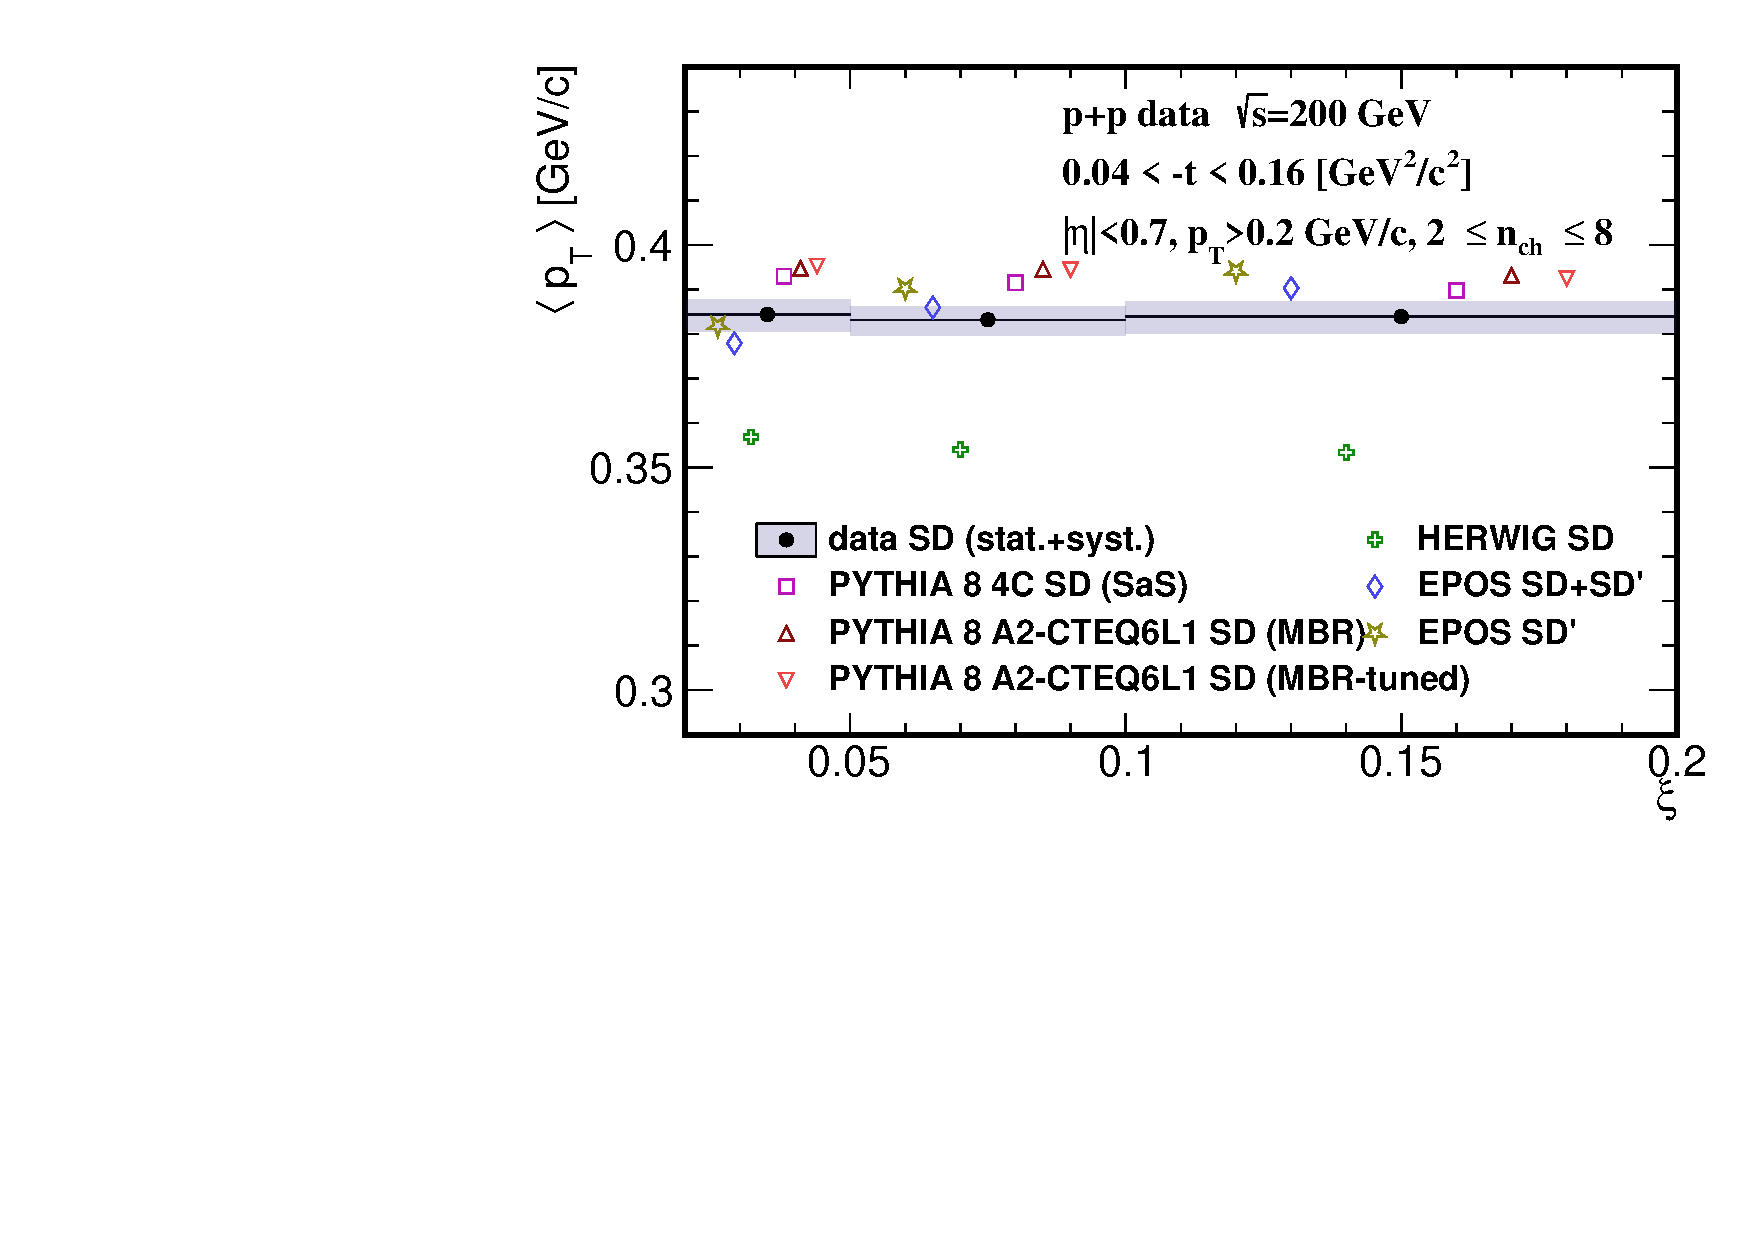
\includegraphics[width=.49\textwidth,page=1]{chapters/chrgSTAR/img/results/mean_pt_xi.pdf}
	%
	\caption{Primary charged-particle multiplicities as a function of $p_\textrm{T}$ shown separately for the~three ranges of  $\xi$: (top left) $0.02<\xi<0.05$, (top right) $0.05<\xi<0.1$, (bottom left) $0.1<\xi<0.2$ and (bottom right) the mean transverse momentum $\langle p_\textrm{T}\rangle$ as a function of $\xi$.}
	\label{fig:results_star_pt}
\end{figure}

Figure~\ref{fig:results_star_pt} shows densities of charged-particles as a function of transverse momentum  $p_\textrm{T}$ in different intervals of $\xi$ and for average values of  $p_\textrm{T}$ in those $\xi$ ranges.
Data show that $\langle p_\textrm{T}\rangle$ depends very weakly on $\xi$. MC models describe data fairly well predicting $\langle p_\textrm{T}\rangle$ only 0.01~GeV/c higher than in data except for the HERWIG SD, which predicts much steeper dependence of particle density on  $p_\textrm{T}$ in all three $\xi$ ranges.


\begin{figure}[t!]
	\centering
	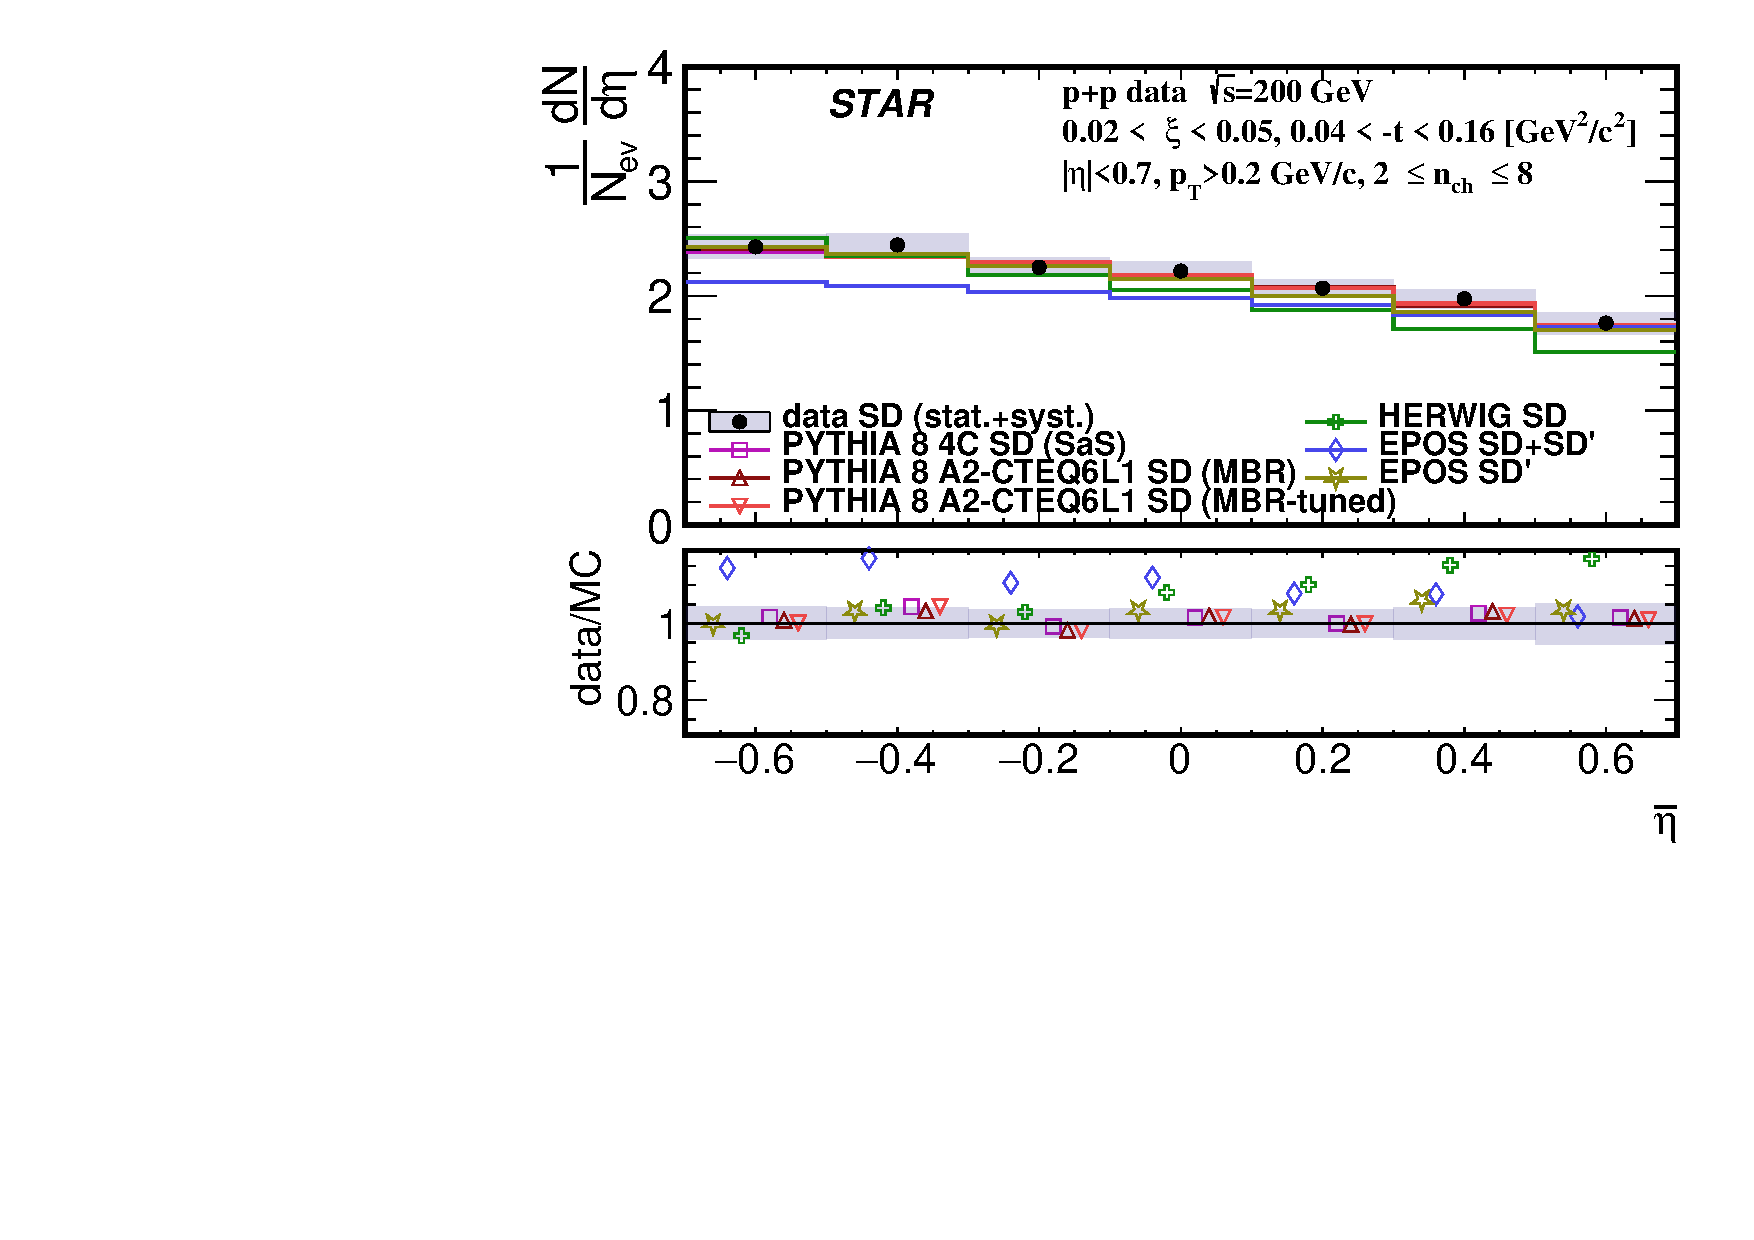
\includegraphics[width=.49\textwidth,page=1]{chapters/chrgSTAR/img/results/out_eta_SD_0.pdf}
	\hfill
	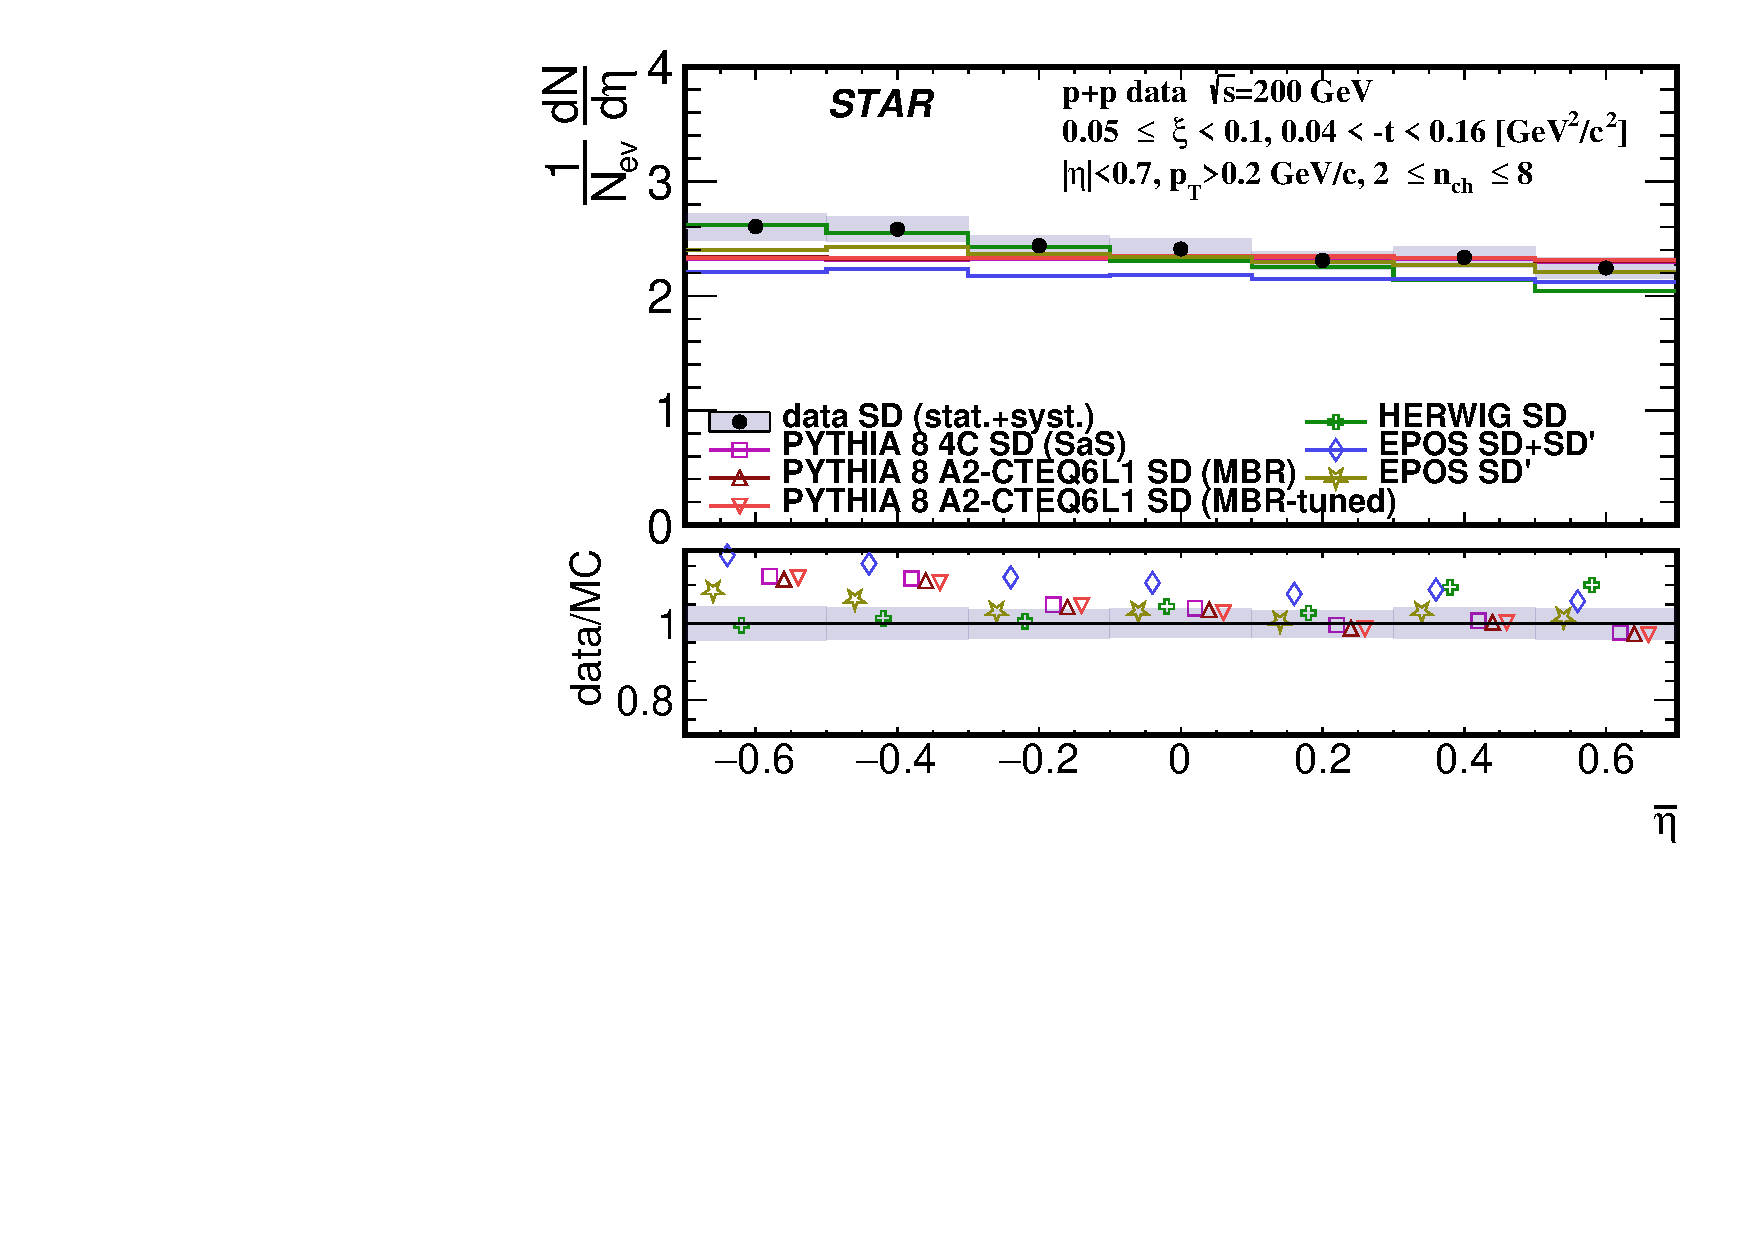
\includegraphics[width=.49\textwidth,page=1]{chapters/chrgSTAR/img/results/out_eta_SD_1.pdf}
	\newline
	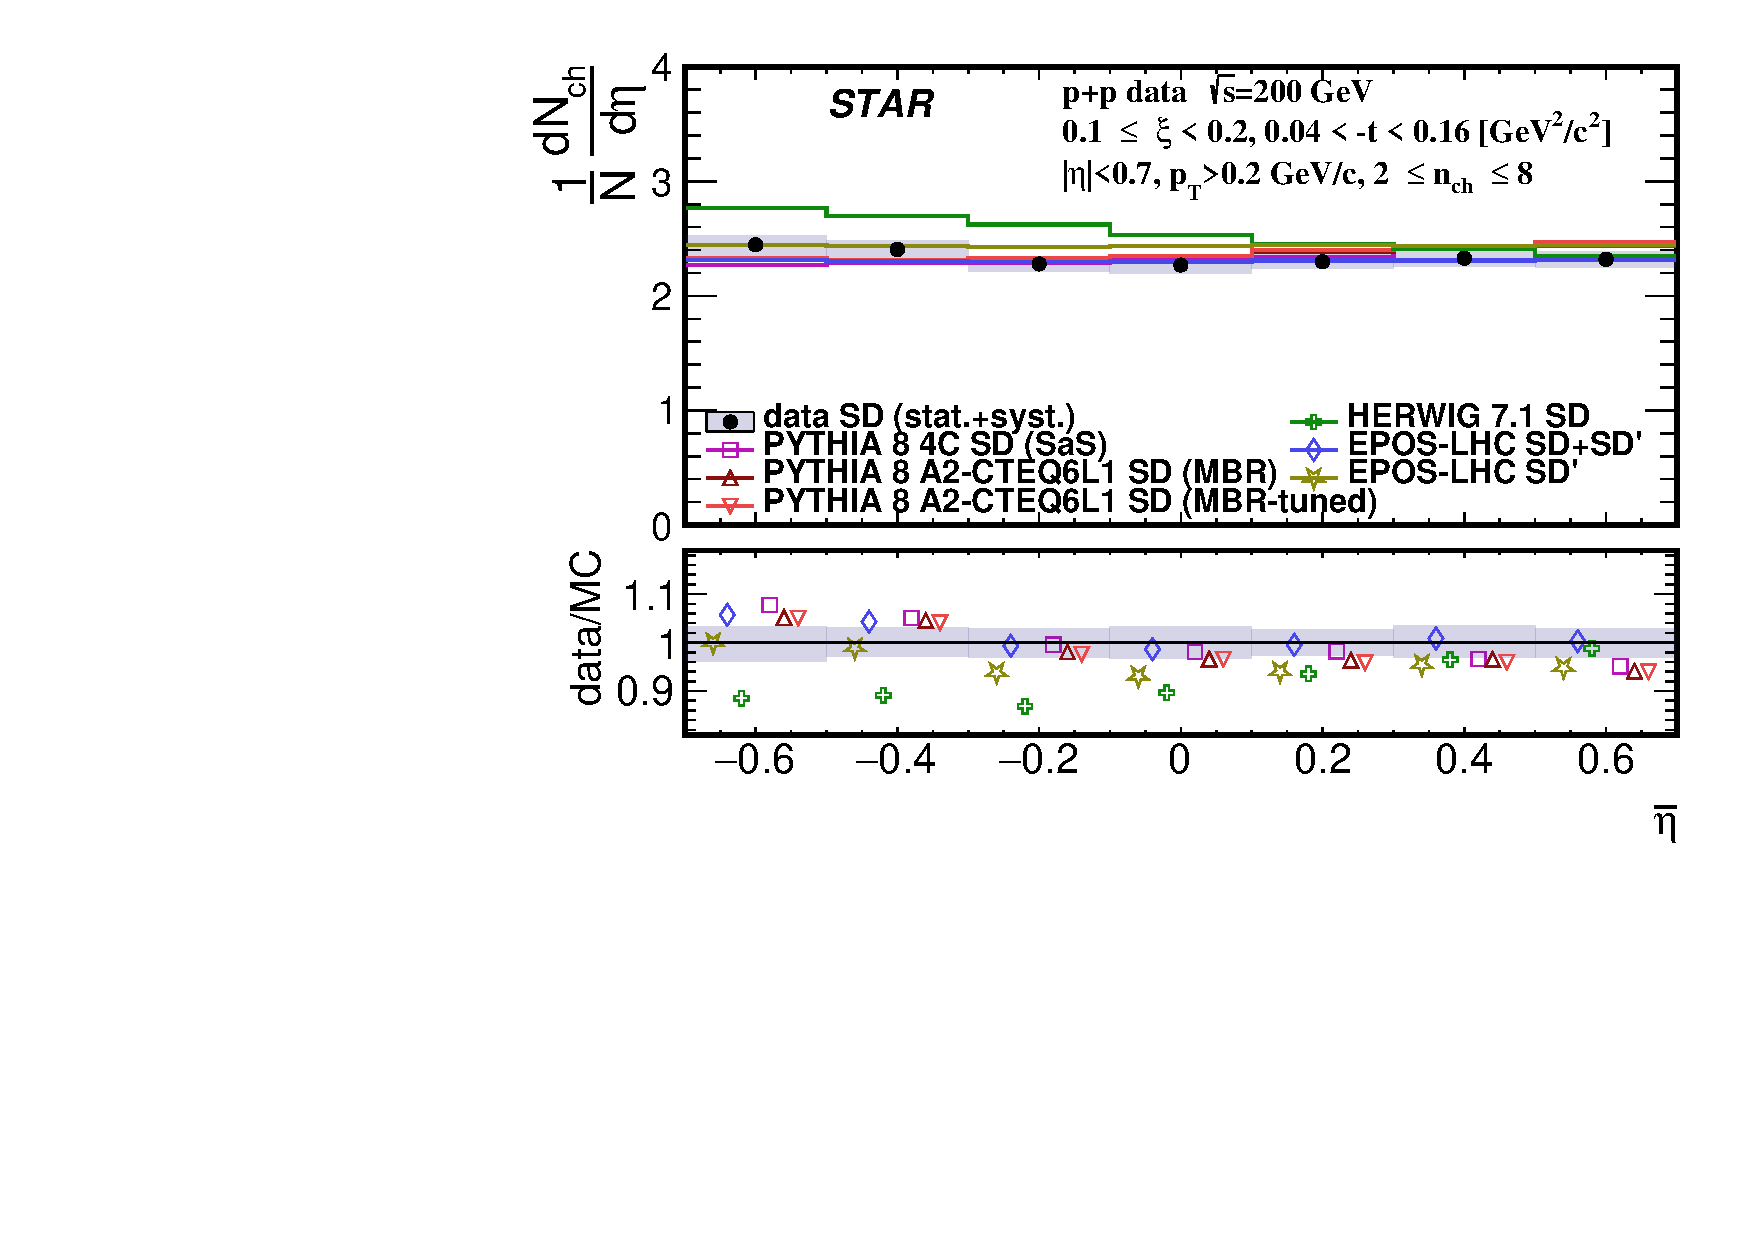
\includegraphics[width=.49\textwidth,page=1]{chapters/chrgSTAR/img/results/out_eta_SD_2.pdf}
	\hfill
	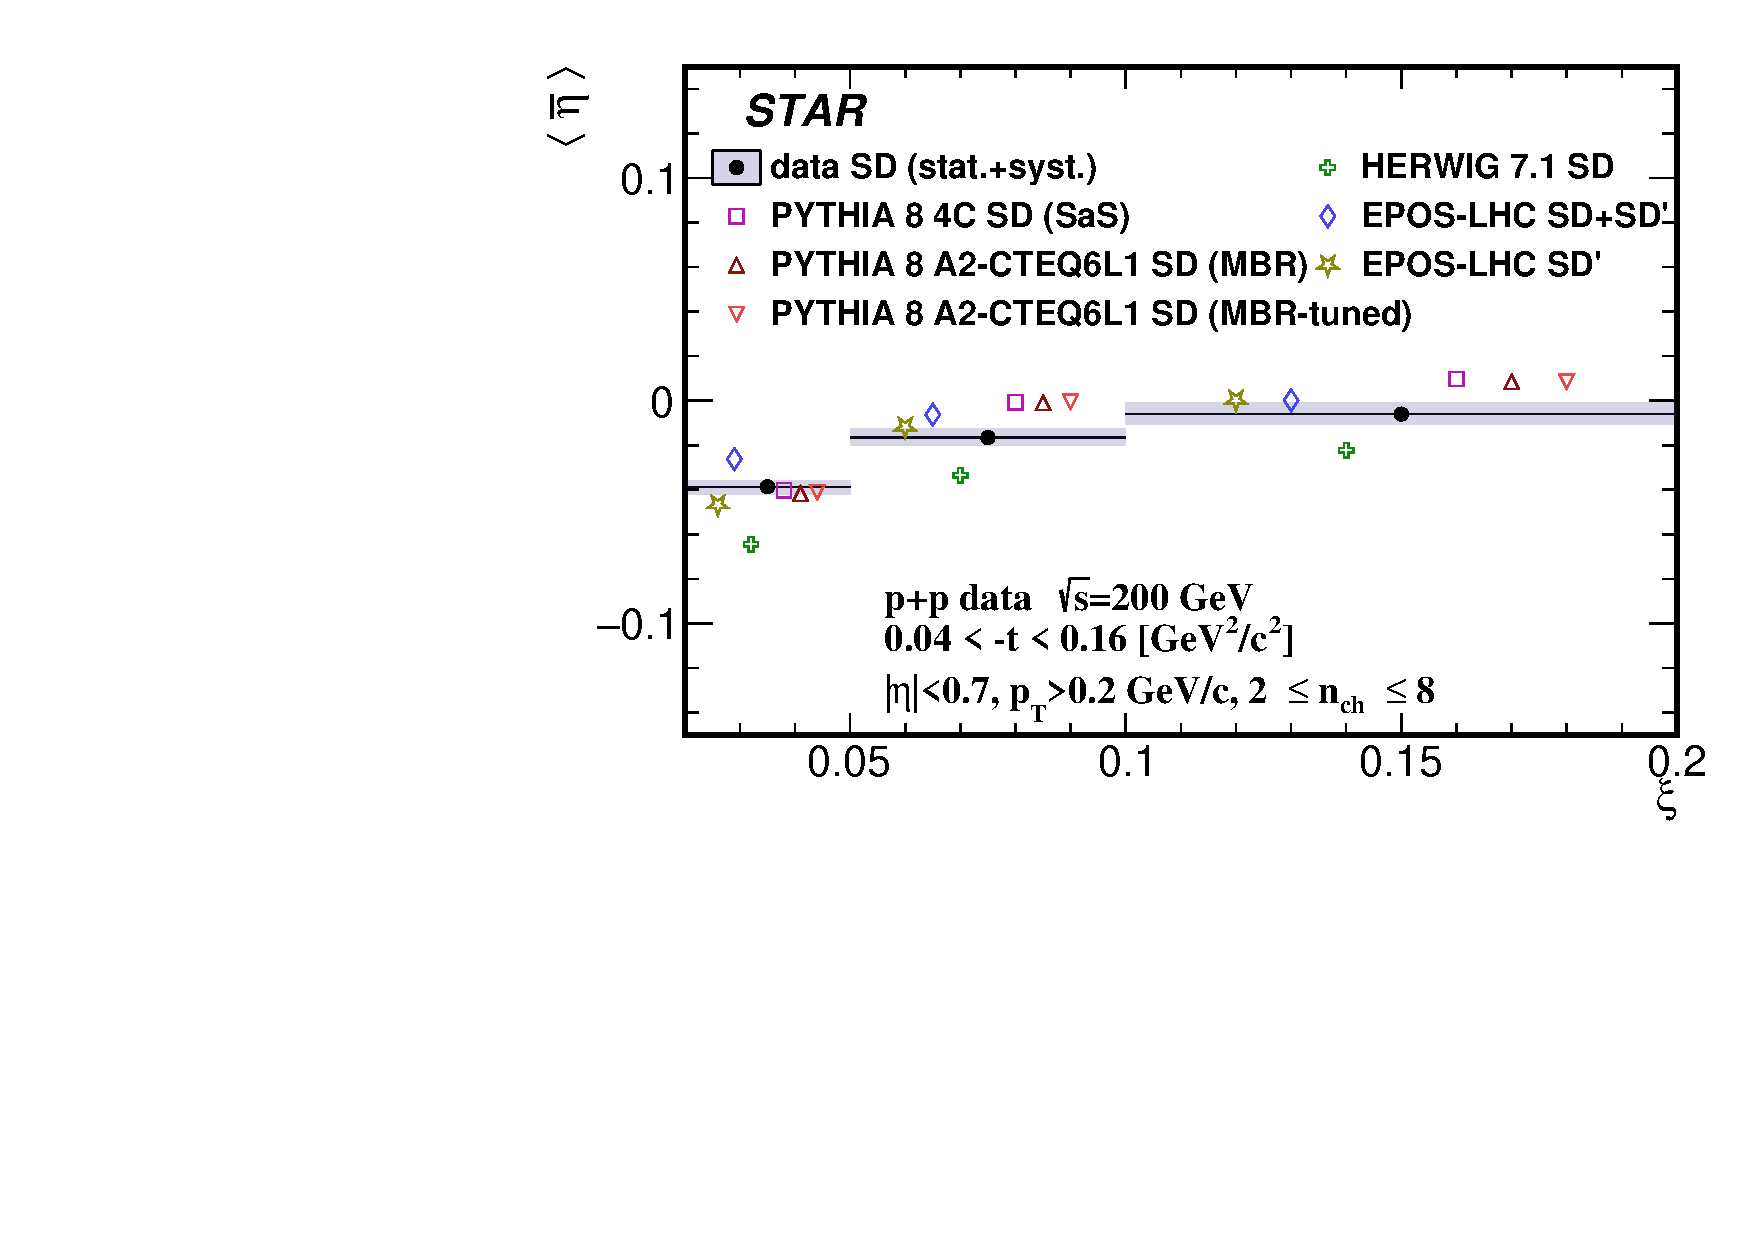
\includegraphics[width=.49\textwidth,page=1]{chapters/chrgSTAR/img/results/mean_eta_xi.pdf}
	%
	\caption{Primary charged-particle multiplicity as a function of $\bar{\eta}$ shown  separately for the~three ranges of  $\xi$: (top left) $0.02<\xi<0.05$, (top right) $0.05<\xi<0.1$, (bottom left) $0.1<\xi<0.2$ and (bottom right) the mean pseudorapidity  $\langle\bar{\eta}\rangle$ as a function of $\xi$.}
	\label{fig:results_star_eta}
\end{figure}

Figure~\ref{fig:results_star_eta} shows densities of  charged-particles as a function of $\bar{\eta}$ in different intervals of $\xi$ and average values of $\bar{\eta}$ in those $\xi$ ranges.
Data show expected flattening of the $\bar{\eta}$ distribution with increasing $\xi$, which reflects SD event-asymmetry and the fact that the position of midrapidity $\eta_m$ at large $\xi$ is closer to the fiducial $|\eta|<0.7$ region, leading to more flat distribution of particle density as a function of $\bar{\eta}$. Models describe data fairly well except EPOS SD+SD$^\prime$, which predicts too flat $\bar{\eta}$ distributions in all three $\xi$ ranges and the HERWIG SD, which predicts too steep $\bar{\eta}$ distributions. Similarly to $n_\textrm{ch}$ distributions  EPOS SD$^\prime$ describes data better compared to EPOS  SD+SD$^\prime$.



\begin{figure}[b!]
	\thisfloatpagestyle{fancy}
	\centering
	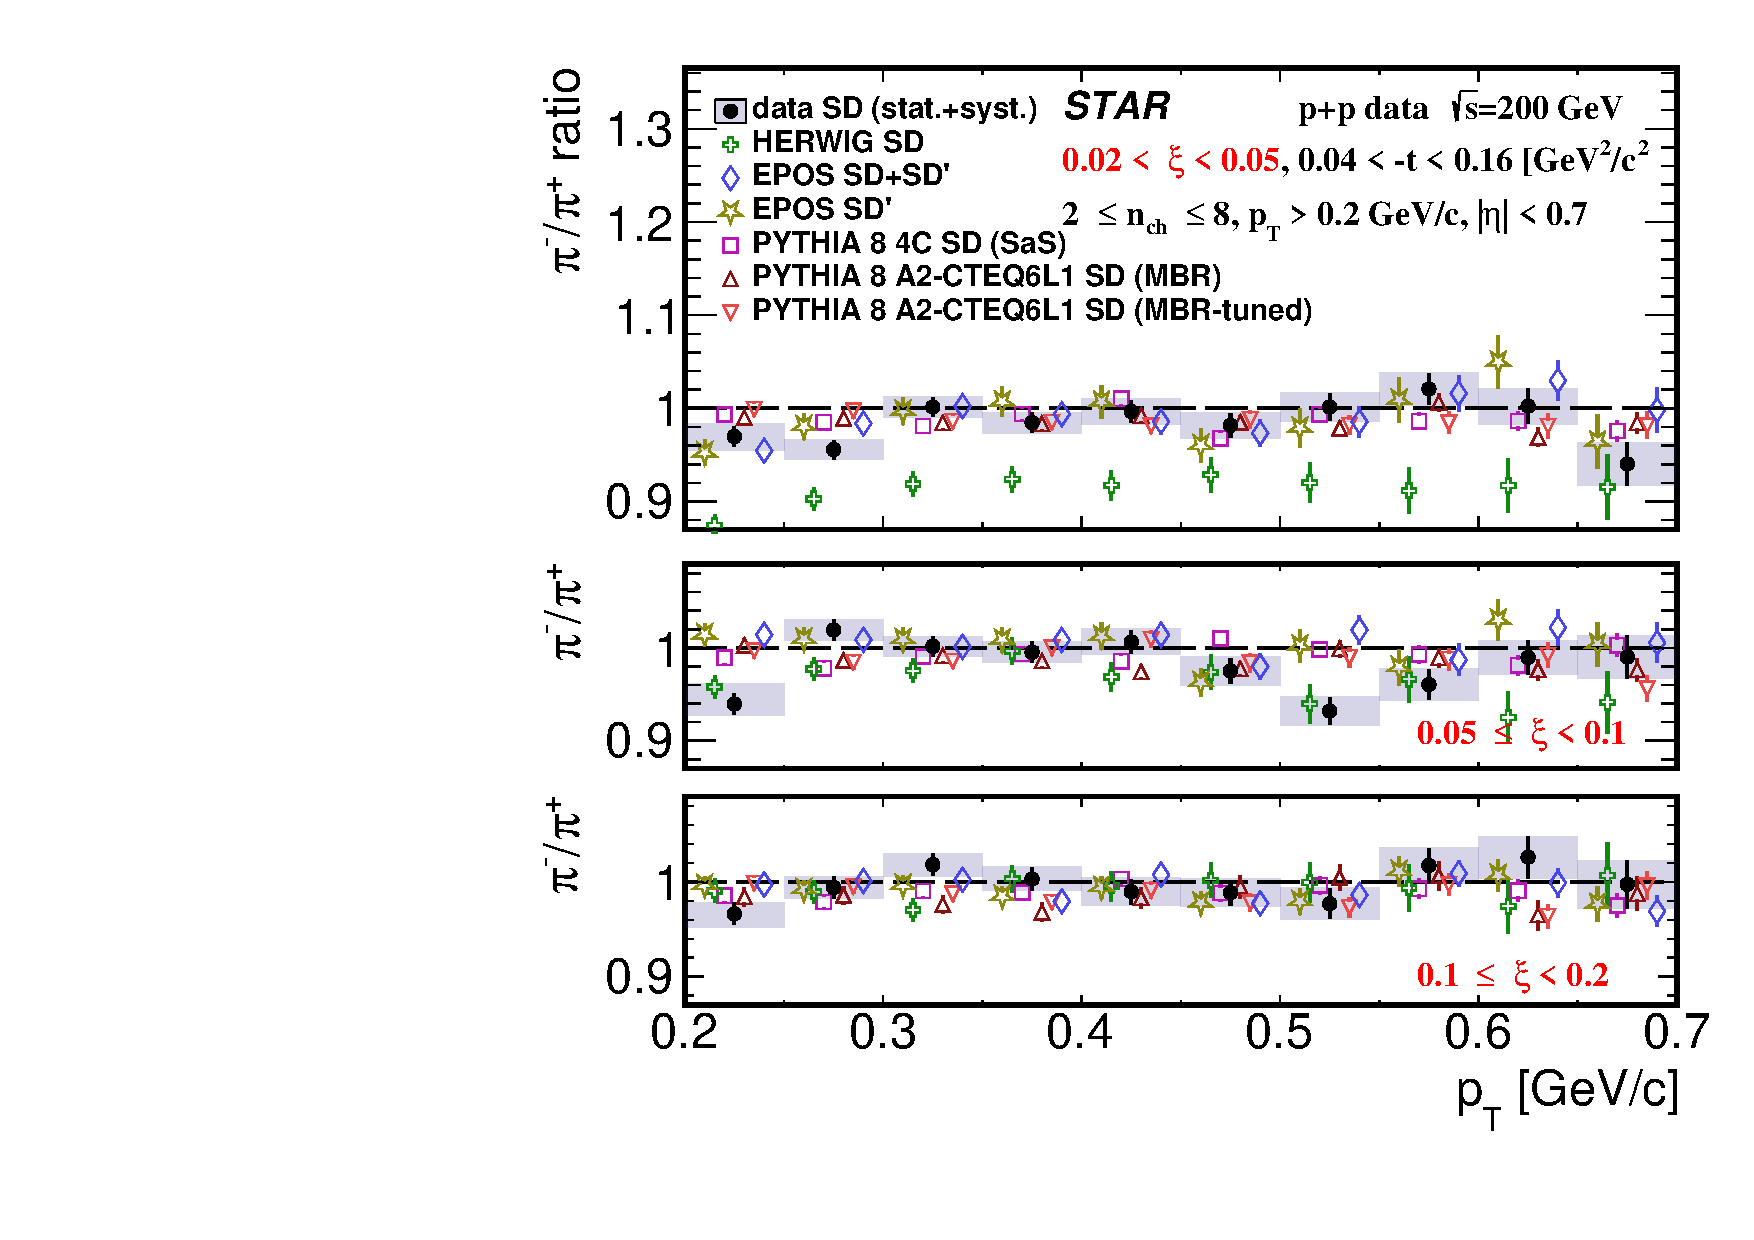
\includegraphics[width=.99\textwidth,page=1]{chapters/chrgSTAR/img/results/particleRatio_prt_0.pdf}
	%
	\caption{Ratio of production yields of $\pi^-/\pi^+$ as a function of $p_\textrm{T}$ shown separately for the~three ranges of $\xi$: (top) $0.02<\xi<0.05$, (middle) $0.05<\xi<0.1$, (bottom) $0.1<\xi<0.2$.}
	\label{fig:results_star_pion}
	
\end{figure}

In Fig.~\ref{fig:results_star_pion} we present the ratios of production yields of $\pi^-/\pi^+$ in three intervals of $\xi$ as a~function of $p_\textrm{T}$.
Data in all three $\xi$ ranges are consistent with equal amounts of $\pi^+$ and $\pi^-$ with no $p_\textrm{T}$ dependence.  MC models agree with data (except HERWIG SD) predicting on average a~small deviation from unity by $\sim 2\%$, which is smaller than the data uncertainties. The model implemented in HERWIG SD, in the first two $\xi$ ranges predicts too large asymmetry between $\pi^+$ and $\pi^-$.

Figure~\ref{fig:results_star_kaon} shows the ratios of production yields of $K^-/K^+$ in three intervals of $\xi$ as a function of $p_\textrm{T}$.
Data in all three $\xi$ ranges are consistent with equal amounts of $K^+$ and $K^-$ with no $p_\textrm{T}$ dependence. Models agree with the data except for HERWIG SD in first $\xi$ range, which predicts too large ratio of $K^-$ to $K^+$.
\begin{figure}[b!]
	\thisfloatpagestyle{fancy}
	\centering
	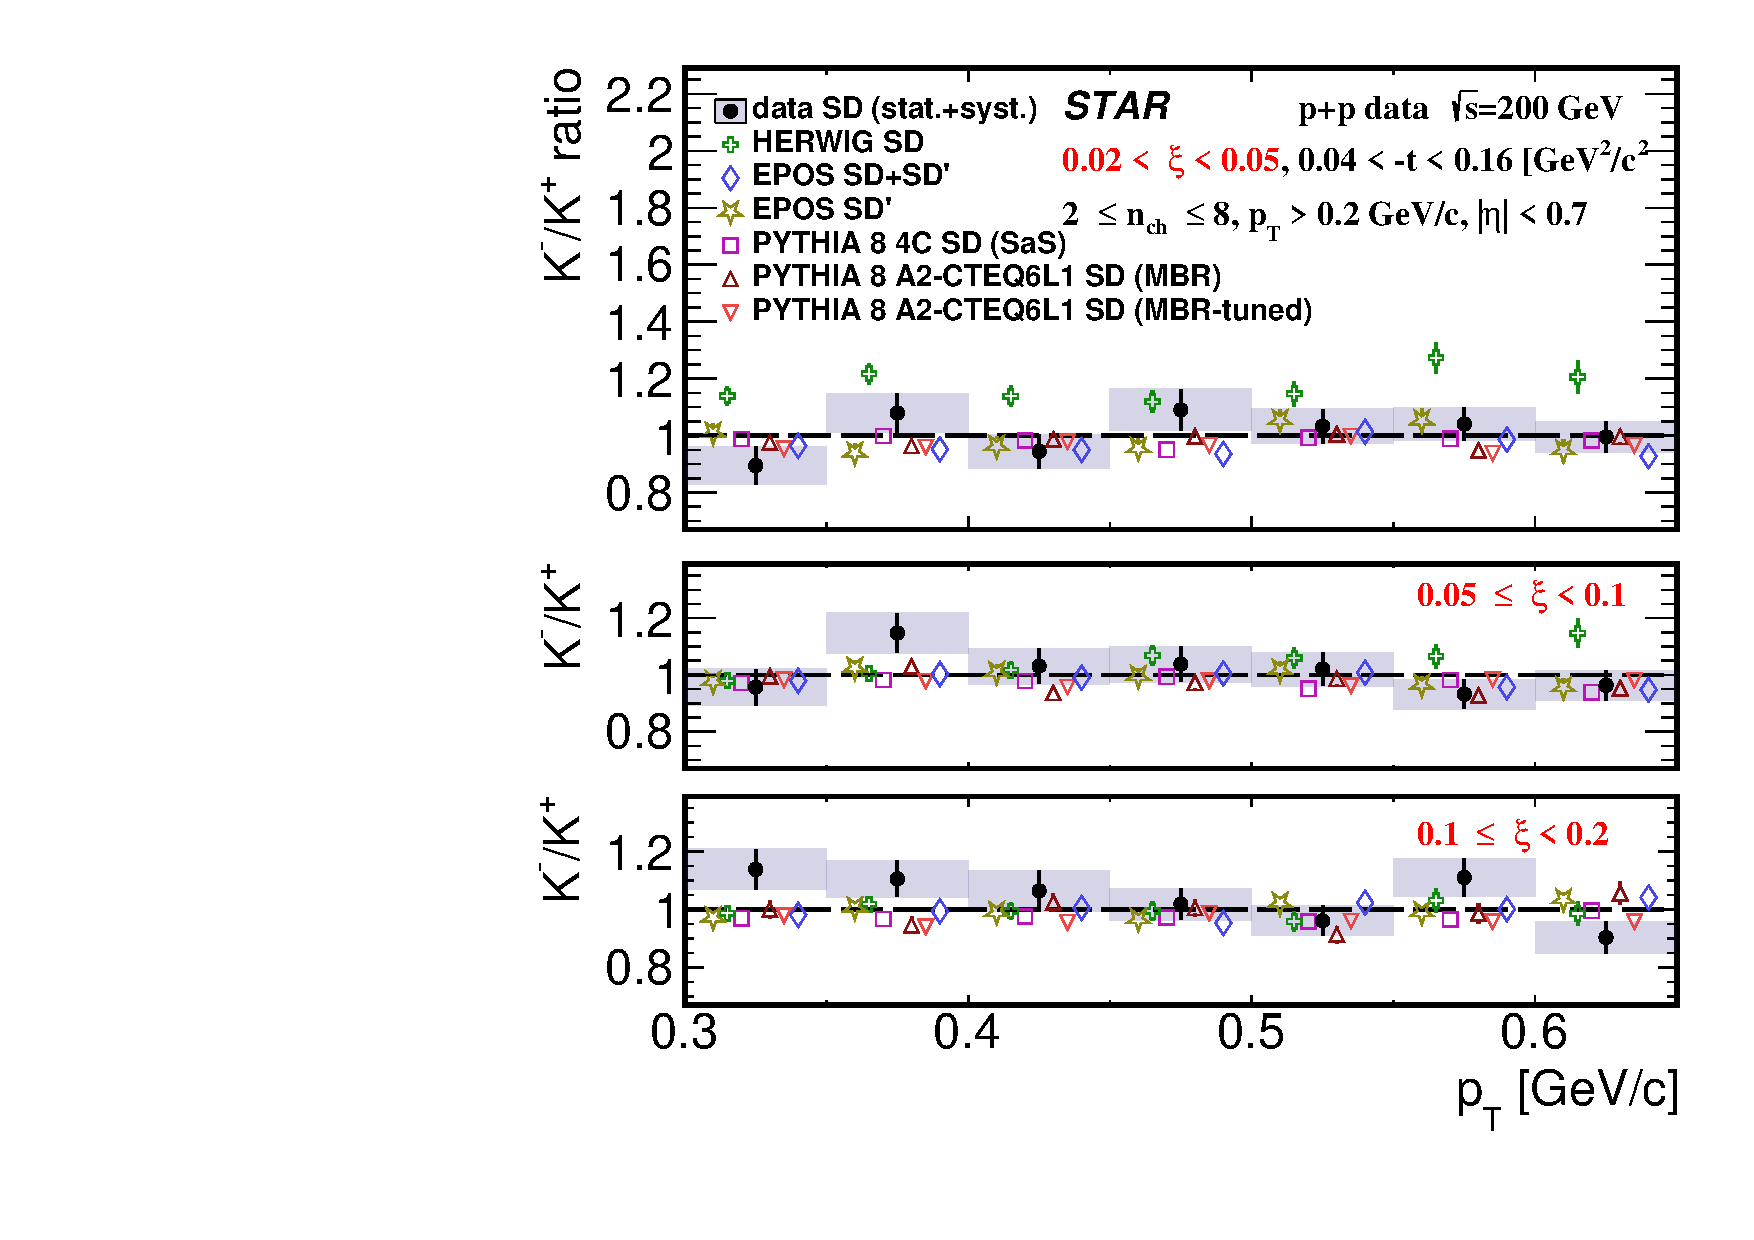
\includegraphics[width=.99\textwidth,page=1]{chapters/chrgSTAR/img/results/particleRatio_prt_1.pdf}
	%
	\caption{Ratio of production yields of $K^-/K^+$ as a function of $p_\textrm{T}$ shown separately for the~three ranges of $\xi$: (top) $0.02<\xi<0.05$, (middle) $0.05<\xi<0.1$, (bottom) $0.1<\xi<0.2$.}
	\label{fig:results_star_kaon}
	
\end{figure}

Figure~\ref{fig:results_star_proton} shows the ratios of production yields of $\bar{p}/p$ in three intervals of $\xi$ as a function of $p_\textrm{T}$.
In the last two $\xi$ ranges, data are consistent with equal amounts of $p$ and $\bar{p}$ with no $p_\textrm{T}$ dependence. However, in the first $\xi$ range at $p_\textrm{T}<0.7$ GeV, data show a significant deviation from unity indicating a large transfer of the baryon number from the forward to the central region.
PYTHIA~8, EPOS SD$^\prime$ and EPOS SD+SD$^\prime$ agree with data in the last two $\xi$ ranges. In the first $\xi$ range, they predict small deviation from unity by $\sim 5\%$, which is smaller than $\sim 15\%$ observed in data. HERWIG SD  predicts much larger baryon number transfer compared to data in all three $\xi$ ranges. This observation is caused by the fact, that HERWIG SD is effectively an extreme realization of the model in which there is almost always a baryon present at gap edge. Significant increase of $\bar{p}/p$ ratio with increasing $\xi$ is related to the fact that the gap edge is further away from the fiducial $\eta$ region at larger $\xi$. EPOS SD+SD$^\prime$ predicts slightly higher baryon number transfer compared to data in first $\xi$ range while EPOS SD$^\prime$ slightly smaller.  This suggests, that $\bar{p}/p$ ratio might be a good observable for tuning relative fractions of SD and SD$^\prime$ processes in EPOS.



Figure~\ref{fig:results_mean_ratio_star} shows the ratios of production yields of $\pi^-/\pi^+$, $K^-/K^+$ and $\bar{p}/p$ integrated over fiducial region in $p_\textrm{T}$ as a function of $\xi$. The results with increased statistical precision confirm conclusions from ratios calculated differentially in $p_\textrm{T}$.


Figure~\ref{fig:results_Kpi_ratio} shows the ratios of production yields of $\left(K^-+K^+\right)/\left(\pi^-+\pi^+\right)$ in three intervals of $\xi$ as a function of $p_\textrm{T}$. The ratio increases from 0.05 at $p_\textrm{T}=0.3$ GeV to $0.22-0.28$ at $p_\textrm{T}=0.65$~GeV. The slope of the $p_\textrm{T}$ dependence significantly increases at $p_T=0.5$ GeV in all three $\xi$ intervals. The change of the $p_\textrm{T}$ slope increases with $\xi$. All models predict very similar $(K^++K^-)/(\pi^++\pi^-)$ ratio except HERWIG, which predicts almost twice larger value independently from $p_\textrm{T}$. PYTHIA~8 and EPOS agree very well with data at $0.3<p_T<0.5$ GeV but do not expect a change of the slope of $p_\textrm{T}$ dependence at $p_\textrm{T}>0.5$ GeV predicting rather almost twice smaller ratio at the highest $p_\textrm{T}$ value.


Figure~\ref{fig:results_Kpi_xi} shows the ratio of the production yields of $\left(K^-+K^+\right)/\left(\pi^-+\pi^+\right)$ as a function of $\xi$ integrated over $0.3<p_\textrm{T}<0.65$ GeV. We do not observe any dependence on $\xi$. PYTHIA~8 and EPOS predictions agree with the data. HERWIG predicts much higher $\left(K^-+K^+\right)/\left(\pi^-+\pi^+\right)$ ratio. 

\begin{figure}[b!]
	\thisfloatpagestyle{fancy}
	\centering
	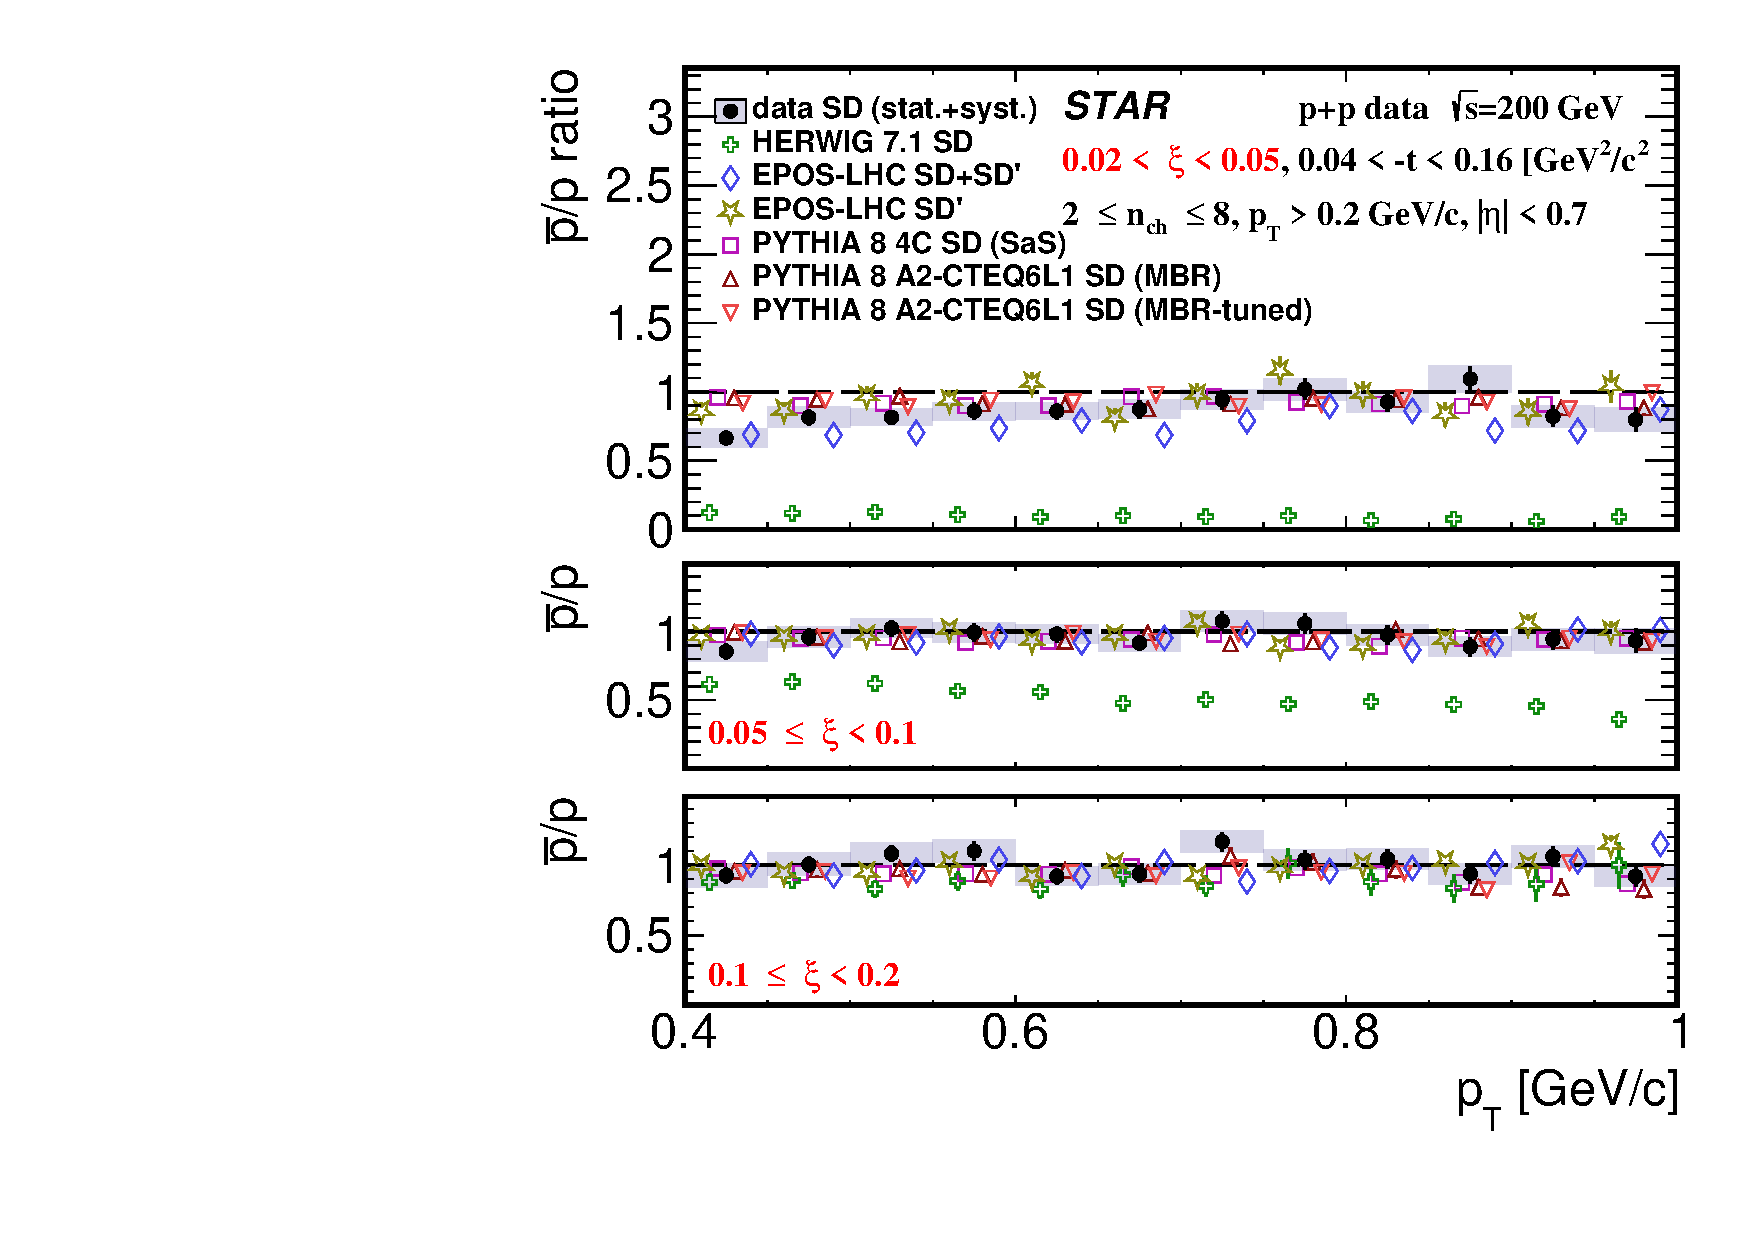
\includegraphics[width=.99\textwidth,page=1]{chapters/chrgSTAR/img/results/particleRatio_prt_2.pdf}
	%
	\caption{Ratio of production yields of $\bar{p}/p$ as a function of $p_\textrm{T}$ shown separately for the~three ranges of $\xi$: (top) $0.02<\xi<0.05$, (middle) $0.05<\xi<0.1$, (bottom) $0.1<\xi<0.2$.}
	\label{fig:results_star_proton}
	
\end{figure}

\begin{figure}[b!]
	\thisfloatpagestyle{fancy}
	\centering
	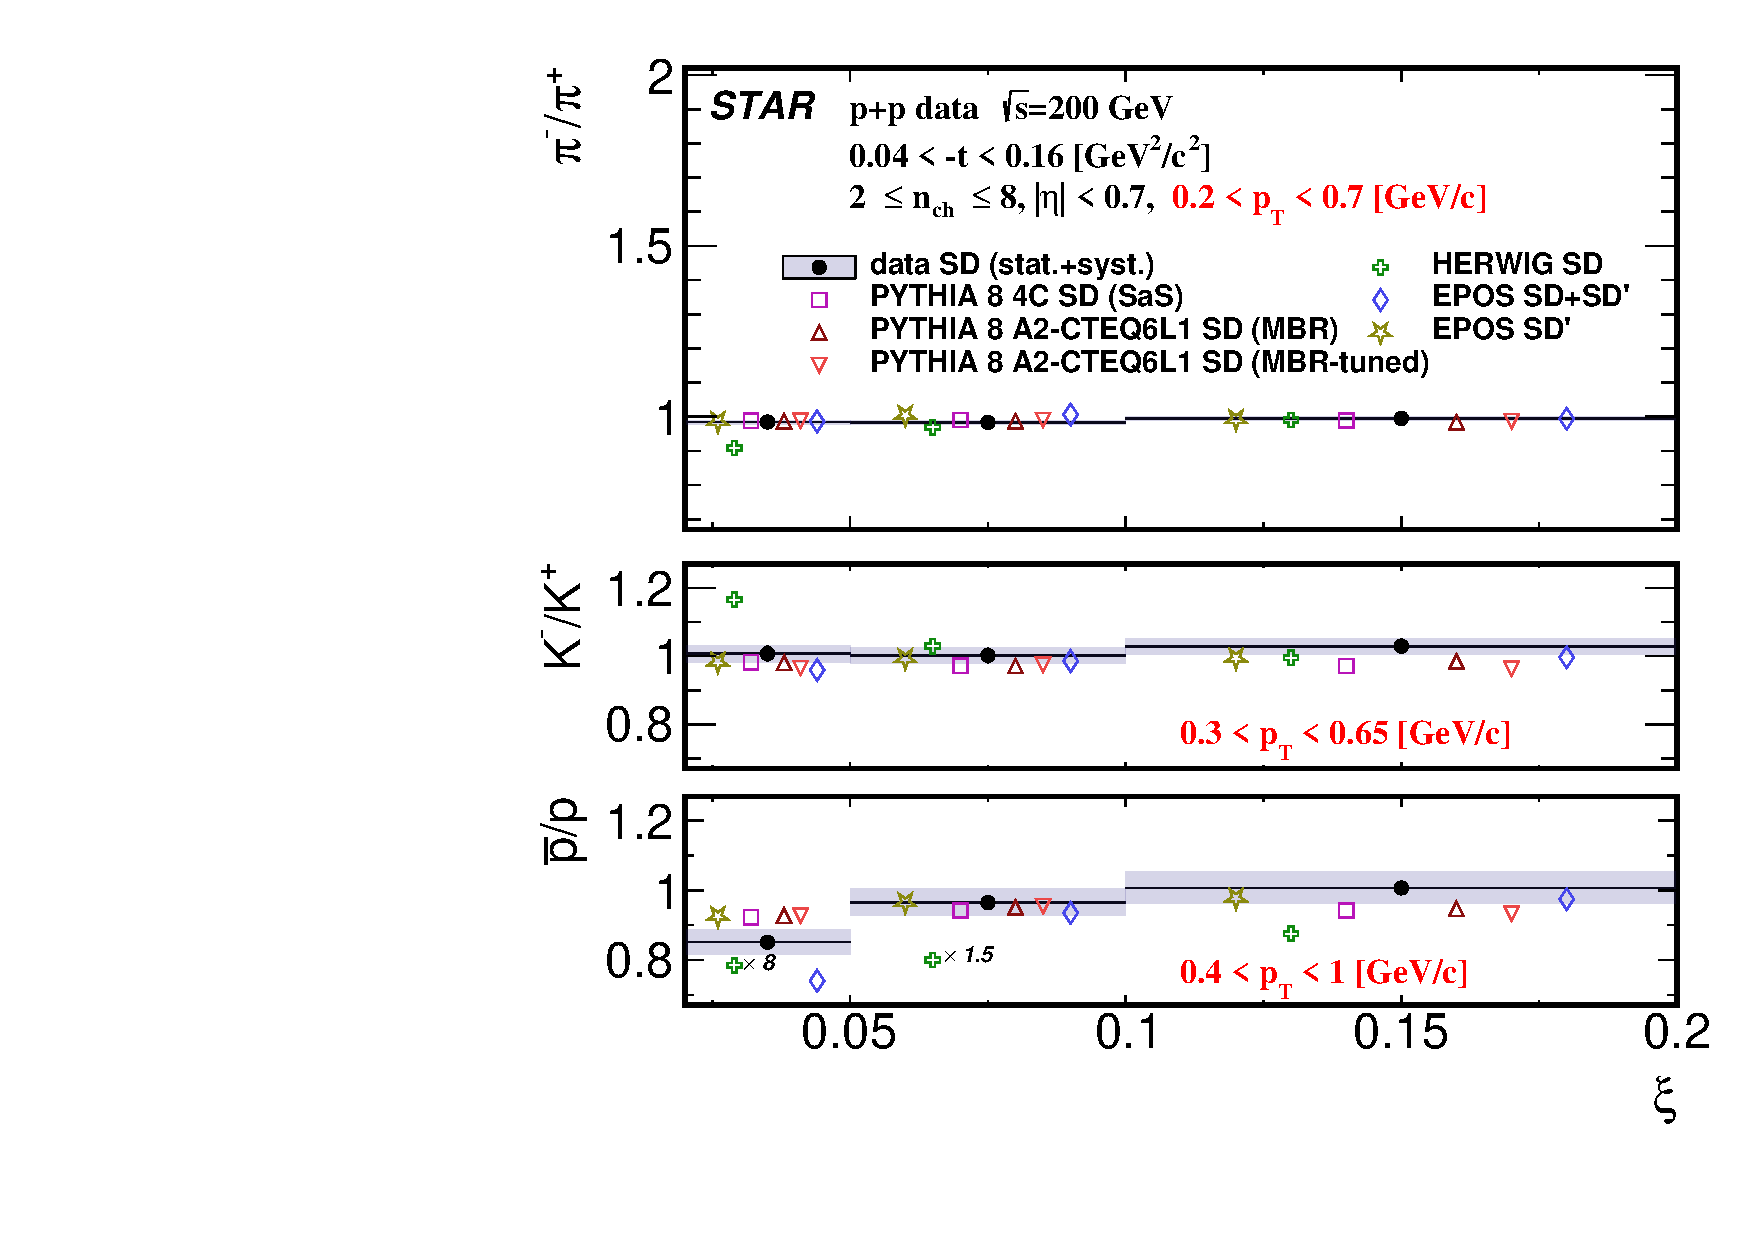
\includegraphics[width=.99\textwidth,page=1]{chapters/chrgSTAR/img/results/ratio_xi.pdf}
	%
	\caption{Ratio of production yields of $\pi^-/\pi^+$, $K^-/K^+$ and $\bar{p}/p$ as a~function of $\xi$. }
	\label{fig:results_mean_ratio_star}
	
\end{figure}

\begin{figure}[b!]
	\thisfloatpagestyle{fancy}
	\centering
	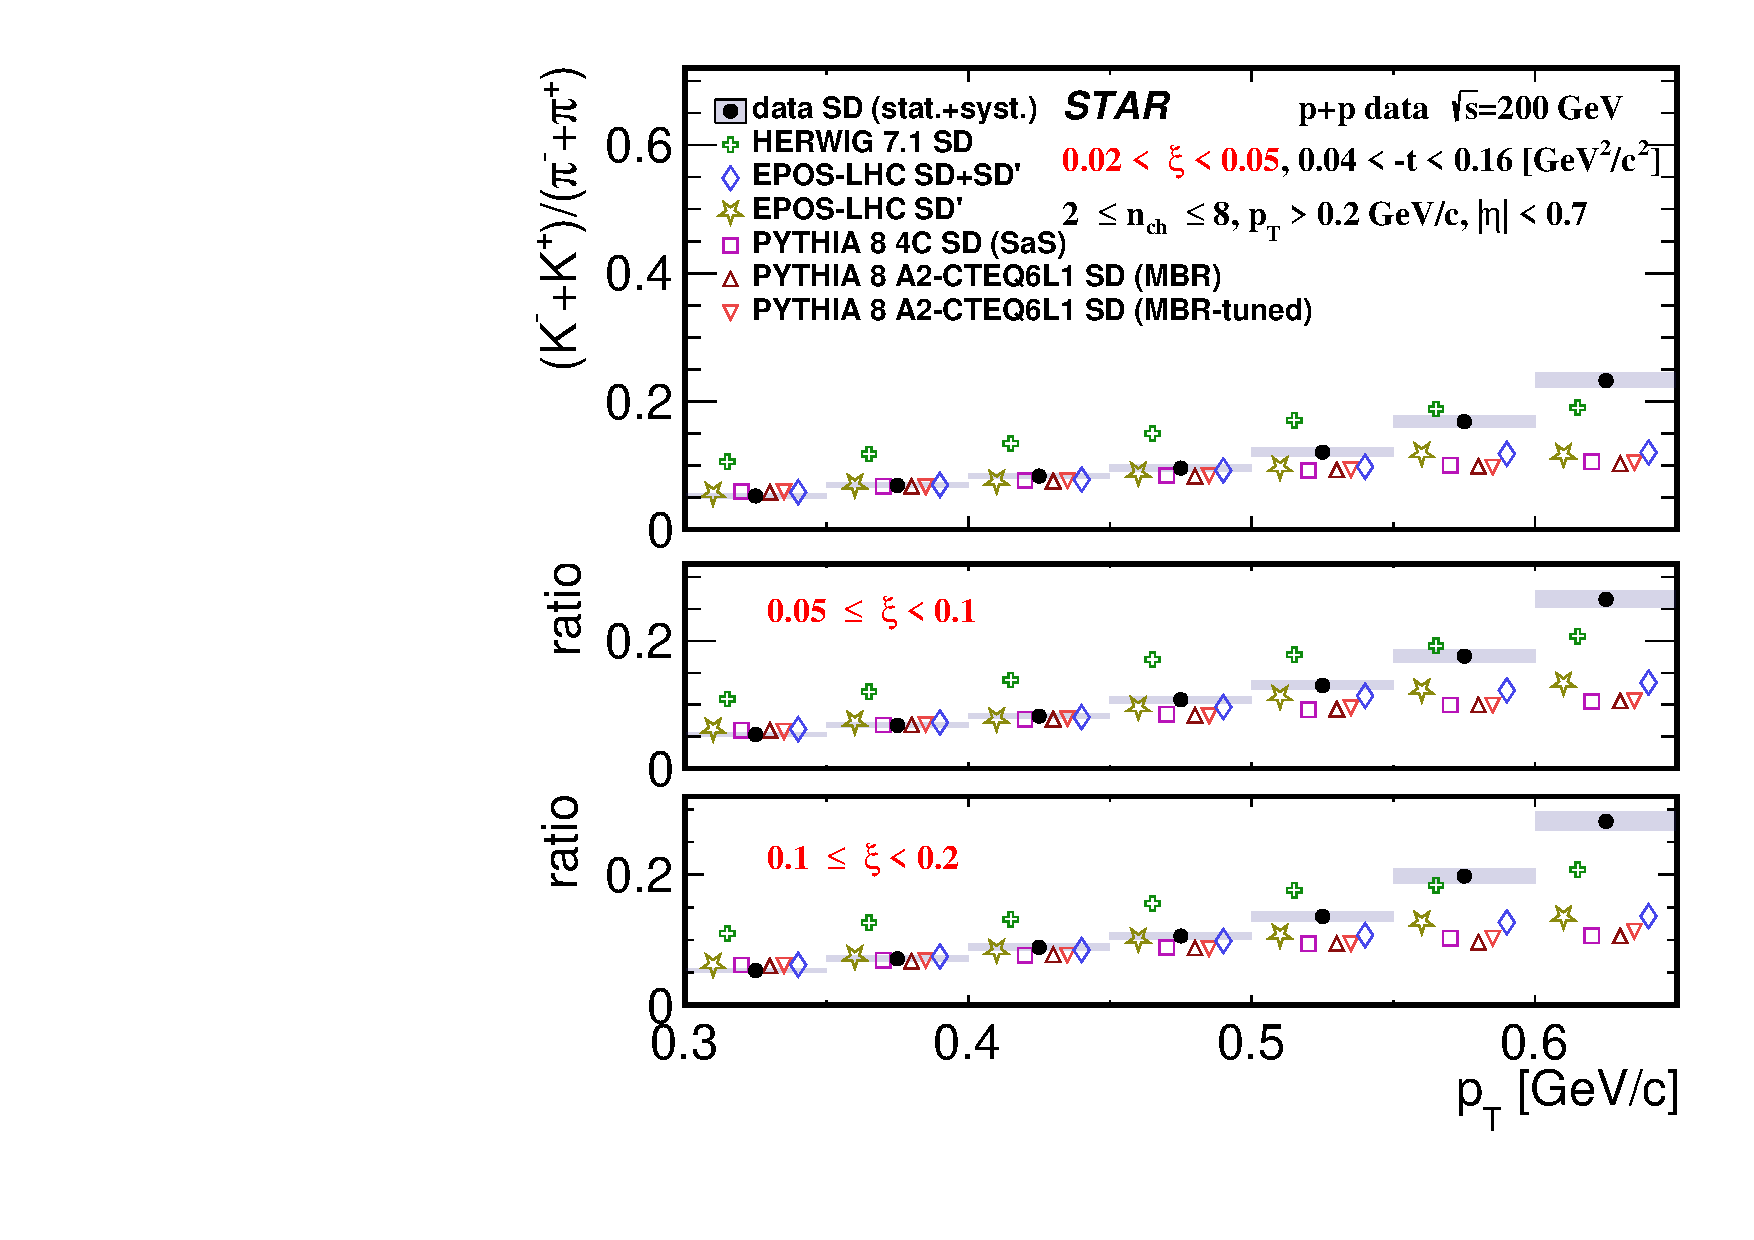
\includegraphics[width=.99\textwidth,page=1]{chapters/chrgSTAR/img/results/particleRatio_Kpi_.pdf}
	%
	\caption{Ratio of production yields of  $\left(K^-+K^+\right)/\left(\pi^-+\pi^+\right)$ as a~function of $p_\textrm{T}$ shown separately for the~three ranges of $\xi$: (top) $0.02<\xi<0.05$, (middle) $0.05<\xi<0.1$, (bottom) $0.1<\xi<0.2$. }
	\label{fig:results_Kpi_ratio}
	
\end{figure}

\begin{figure}[b!]
	\thisfloatpagestyle{fancy}
	\centering
	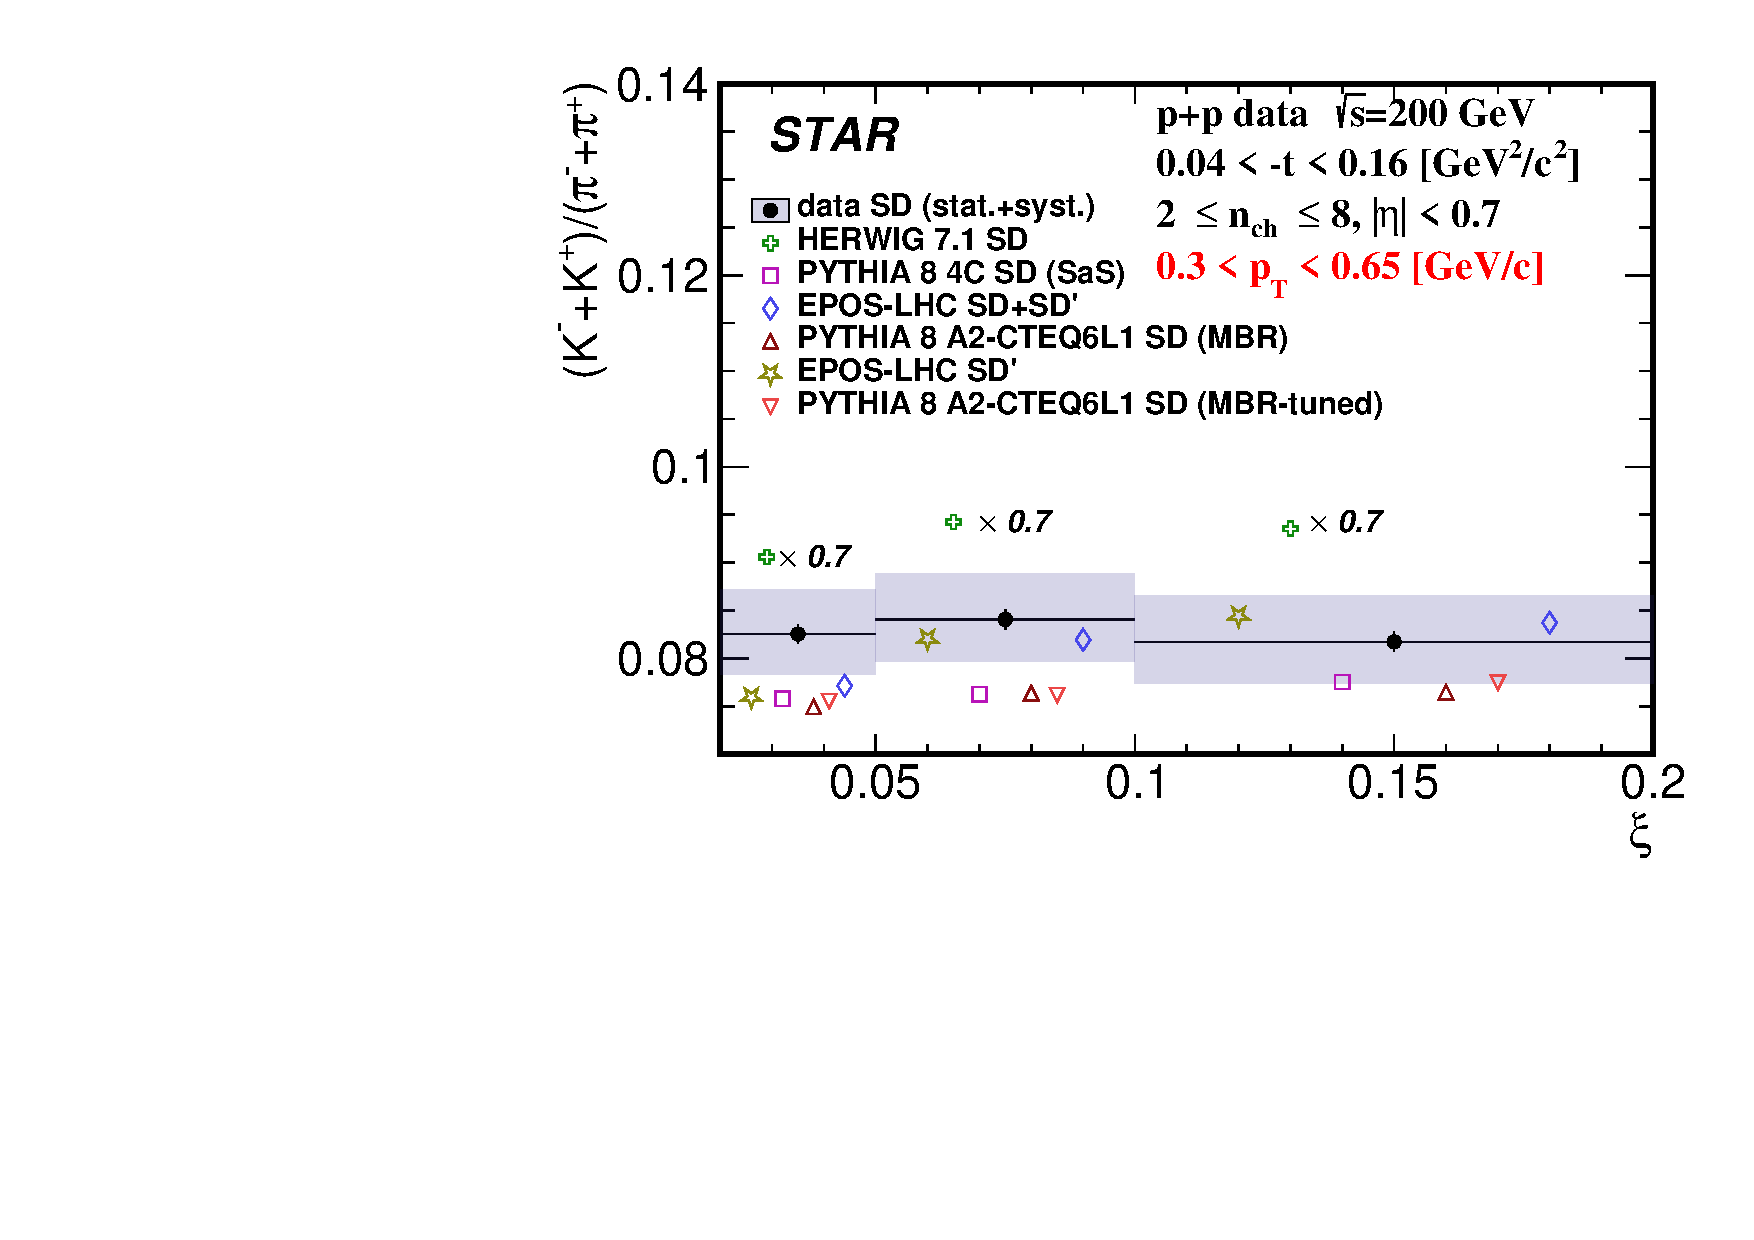
\includegraphics[width=.99\textwidth,page=1]{chapters/chrgSTAR/img/results/outPID_Kpi_ratio_xi.pdf}
	%
	\caption{Ratio of production yields of $\left(K^-+K^+\right)/\left(\pi^-+\pi^+\right)$ as a~function of $\xi$. }
	\label{fig:results_Kpi_xi}
	
\end{figure}

\FloatBarrier